\documentclass[a4paper]{article}   % On declare le type du document : article, book, beamer (pour une presentation)... %  a4paper car c'est le format standard du papier en Europe.

%%%% Packages

\usepackage{lmodern}
\usepackage[french]{babel}  		% on écrit en français
\usepackage[utf8x]{inputenc} 		% pour utiliser toutes les touches du clavier
\usepackage[T1]{fontenc}  		% pour utiliser toutes les touches du clavier
\usepackage{pifont}
\usepackage[dvips]{graphicx}  		%Pour Compiler en LaTeX    %%%%%%%%
\usepackage{graphics}        		% Pour Compiler en LaTeX    %%%%%%%% ATTENTION!!!! pour sortir du TeXgraph en pdf il faut le package graphicx dans le préambule et includegraphics{*.pdf} dans le dodument. Mais cela fait foirer la compilation LaTeX.
\usepackage[dvips]{graphicx}        	%pour le pdf
\usepackage{multirow}
\usepackage{epsfig}			% Pour importer une image
\usepackage{variations}  			% Tableaux de variations

\usepackage{minibox}
\usepackage{marvosym}
%\usepackage{hyperref}
\usepackage{enumerate}
\usepackage{wrapfig}
\usepackage{multicol}
\usepackage{framed}
\usepackage{verbatim}
\usepackage[mathcal,mathscr]{eucal} 
\usepackage{eufrak}
\usepackage[np]{numprint}
\usepackage{tabularx}
\usepackage{fancybox}
\usepackage{amsmath,amsfonts, amssymb}  % Des pack de l'AMS tres utiles en math
\usepackage{lmodern}           		% Ameliore la mise en page des textes francais 
\usepackage{enumerate}         		% Pour faire des listes numerotees.
\usepackage[colorlinks=true,urlcolor=blue]{hyperref} % Liens hyper-textes ...% ...utiles pour un document en ligne,
\usepackage{color}    	% Pour écrire en couleur:  {\color{red} bla} ou {\color[rgb]{0,0,1} bla} [red, green, blue]		
\usepackage{amsthm}
\usepackage[a4paper]{geometry}    	% pour aggrandir ou diminuer les marges.                           
\geometry{a4paper,left=2cm,right=2cm,top=1cm,bottom=1.5cm}

\renewcommand\thesection {\Roman{section}-}	% pour avoir les sections en grec
\renewcommand{\(}{\left(}
\renewcommand{\)}{\right)}
\newcommand{\e}{\,\text{e}\,} 
\newcommand{\limit}[2]{\lim\limits_{#1 \to #2}}

%%%

\definecolor{CouleurA}{rgb}{0, 0, 0} %noir
\definecolor{CouleurB}{rgb}{0.77751, 0.2511, 0.13799}
\definecolor{CouleurC}{rgb}{0.85895, 0.93161, 0.10727}
\newenvironment{TraitV}[3][CouleurA]{%
% #1 couleur du trait (par défaut CouleurA)
% #2 largeur du trait
% #3 distance entre le trait et le texte
\def\FrameCommand{{\color{#1}\vrule width #2}
\hspace{#3}}%
\MakeFramed {\advance\hsize-\width}}%
{\endMakeFramed}

%%%

\renewcommand{\theenumi}{\textbf{\arabic{enumi}}}
\renewcommand{\labelenumi}{\textbf{\theenumi.}}
\renewcommand{\theenumii}{\textbf{\alph{enumii}}}
\renewcommand{\labelenumii}{\textbf{\theenumii.}}

%%%% Théorèmes Français numérotés

\newtheorem{de}{Définition}		% Syntaxe : \begin{de} la li la la \end{de} .
\newtheorem{theom}{Théorème}
\newtheorem{propo}{Propriété}
\newtheorem{que}{Question}
\newtheorem{ques}{~}
\newenvironment{qu}{\begin{ques}--} {\end{ques}}
\newtheorem{rmq}{Remarque}
\newtheorem{exm}{Exemple}
\newtheorem{exoit}{Exercice}
\newenvironment{exo}   {\begin{exoit} \normalfont}
               {\end{exoit} \medskip}			% Les exercices ne seront pas en italique.
\newtheorem{EXO}{\large EXERCICE }
\newenvironment{EX}   { \setcounter{ques}{0} \begin{EXO} \hrulefill ~\vspace{0.3cm}

\normalfont}    {\end{EXO} \medskip}			
\newenvironment{ex}   {\begin{exm} \normalfont}
               {\end{exm} \medskip}			% Les exemples ne seront pas en italique.
\newtheorem*{demo*}{Démonstration}		
\newenvironment{dem}   {\begin{demo*}\normalfont : \begin{TraitV}{1.5pt}{10pt}} 
               {\end{TraitV}\end{demo*}\medskip}	
\newenvironment{thm}{\begin{Sbox}\begin{minipage}{0.9\linewidth}\begin{theom} ---}		% les théorèmes seront encadrés.
{\end{theom}\end{minipage}\end{Sbox}\begin{center}\fbox{\TheSbox}\end{center}}
\newenvironment{prop}{\begin{Sbox}\begin{minipage}{0.9\linewidth}\begin{propo} ---}		% les propriétés seront encadrées.
{\end{propo}\end{minipage}\end{Sbox}\begin{center}\fbox{\TheSbox}\end{center}}
%%%%  Nouveaux opérateurs.

\DeclareMathOperator{\diver}{\operatorname{div}}
\DeclareMathOperator{\rot}{\operatorname{rot}}
\DeclareMathOperator{\supp}{\operatorname{Supp}}
\DeclareMathOperator{\conv}{\operatorname{Conv}}

%%%% Raccourcis 
% Par exemple, quand on tapera \R, le code comprendra \mathbb R  qui utilise la bonne police pour écrire l'ensemble des reels.

\newcommand{\R}{ ${\mathbb R} ~$}
\newcommand{\C}{ ${\mathbb C} ~$}
\newcommand{\Z}{ ${\mathbb Z} ~$}
\newcommand{\N}{ ${\mathbb N} ~$}
\newcommand{\Nn}{ ${\mathbb N^*} ~$}
\newcommand{\divpart}[1]{{\displaystyle \frac{\partial #1}{\partial t}}}
\newcommand{\divdroite}[1]{{\displaystyle \frac{d #1}{ dt}}}
\newcommand{\ep}{{\varepsilon}}
\newcommand{\ddt}{{\frac{d}{dt}}}
\newcommand{\dronde}{ {\frac{\partial}{\partial t} }}
\newcommand{\cf}{$\mathcal{C}~$} 	%courbe Cf
\newcommand{\df}{$\mathcal{D}~$} 	%ensemble de définition Df
\newcommand{\ie}{\leqslant ~}  		% pr < ou= et > ou=
\newcommand{\se}{\geqslant~} 		% pr < ou= et > ou=
\newcommand{\ri}{$\left(O;\vec{i};\vec{j}\right)$}
\newcommand{\rIJ}{$\left(O\,;\,I\,;\,J\right)$}
\newcommand{\ru}{$\left(O;\vec{u};\vec{v}\right)$} 	% repères
\newcommand{\f}{\dfrac} 	% =\dfrac = \frac avec displaystyle
\def\v{\overrightarrow}	% vecteur : syntaxe : $\v{AB}$
\newcommand{\al}{\quad \Rightarrow \quad}	% implication
\newcommand{\ssi}{\quad \Leftrightarrow \quad}	% équivalence
\newcommand{\ass}{\mapsto~}		% flèche de "fonction qui a x associe..."
\newcommand{\x}{\times} %pour le symbole x

% \lim\limits_{n \to +\infty} v_n=+\infty  ; limite
% Type de document - classe - date [à faire avec mise en page]

\def\dev{\Large Nombres, ensembles, intervalles}		% Titre chapitre
%\def\dev{DS de mathématiques n°}
%\def\dev{DM de Mathématiques n°}
%\def\dev{Correction des Exercices - Fonctions Trinômes}
%\def\dev{Correction du DM n°}
%\def\dev{ Test de math}
%def\dev{ Autre }
%\def\numero{10}                         % Numéro du devoir
\def\cl{{\Large \bf{2nde}}} 
\def\jour{le 25/09/2020}                  % Date

%%%%%%%%%%%%%%%%%%%%%%%%%%%%%%%%%%%%%%%%%%%%%%%%
%%%%%%%%%%%%%%%%%%%%%%%%%%%%%%%%%%%%%%%%%%%%%%%%
%%%%%%%%%%%%%%%%%%%%%%%%%%%%%%%%%%%%%%%%%%%%%%%%

\begin{document}			% Le document commence ici.


\noindent\begin{minipage}{.20\linewidth}\begin{center}                   
\noindent \emph{Lycée Paul Lapie - Courbevoie}
\end{center}\end{minipage}
\begin{minipage}{1.5\linewidth}\begin{center}		
\noindent \cl\\ Chapitre 1
\end{center}\end{minipage}

\begin{center}\shadowbox{ \Large Planche n°1 : Nombres, ensembles, intervalles } 	
\end{center}

\begin{EX}
\begin{center}
\begin{tabular}{|p{4cm}| p{4cm}| p{4cm}|}		
\hline							
Droite des réels & Inégalités & Intervalles \\
\hline
&& \\
& \qquad $2 \ie x < 9$ &\\
&& \\
\hline
&& \\
& & $\quad ]-\infty\,;\,3]\cup]5\,;\,7[$\\
&& \\
\hline
&& \\
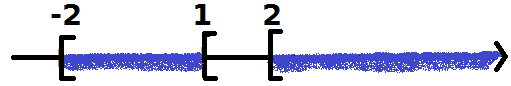
\includegraphics[width=3.9cm]{1ex1.png}&&\\
&&\\
\hline
&& \\
& \qquad $x \se -7 $ &\\
&& \\
\hline
\end{tabular}
\end{center}
\end{EX}

\begin{EX} Dans chaque cas, donner la distance entre les deux nombres réels proposés :
\begin{enumerate}
\item $-2$ et $-12$.
\item $5$ et $-8$.
\item $-\pi$ et $3 \pi$.
\item $-\f{7}{3}$ et $\f{5}{6}$.
\end{enumerate}
\end{EX}
\begin{EX} Déterminer les réels $x$ vérifiant ces égalités : ( = résoudre les équations)
\begin{enumerate}
\item $|x|=8$
\item $|x|=-4$
\item $|x-4|=3$
\item $|6-3x|=4$
\end{enumerate}
\end{EX}
\begin{EX} Quel est le plus petit intervalle auquel appartient $x$ dans chacun des cas suivant ? ( = résoudre les inéquations)
\begin{enumerate}
\item $|x| \ie 5$
\item $|x| > 0 $
\item $|x-3| \ie 4$
\item $|8-2x| \se 2$
\end{enumerate}
\end{EX}
\begin{EX} Compléter les pointillés par $\in \quad \notin \quad \subset \quad \not\subset$ 
$$ -\pi \, .... \,]-5 \,;\, -2] \qquad -5 \,.... \,\mathbb{Z} \qquad \mathbb{Q} \,....\, \mathbb{D} \qquad ]1\,;\, 2] \,....\, [1 \,;\,2] \qquad ]-2 \,;\, 3[ \, .... \, [- \pi \,;\, \pi]\qquad \f{7}{6}\, ....\, \mathbb{D} $$ ~~
$$ \sqrt2 \, .... \,]\f{3}{2} \,;\, -\infty[ \qquad ]-4\,;\, -2] \,....\, ]-\infty \,;\,0[\qquad -5 \,.... \,\mathbb{D} \qquad \mathbb{N} \,....\, \mathbb{D}  \qquad ]3\pi \,;\, 4\pi[ \, .... \, [9 \,;\, 12]\qquad \f{-8}{9}\, ....\, \mathbb{Q}  $$
\end{EX}

\newpage \setcounter{EXO}{0}
\noindent\begin{minipage}{.20\linewidth}\begin{center}                   % Lycée en haut à droite
\noindent \emph{Lycée Paul Lapie - Courbevoie}
\end{center}\end{minipage}
\begin{minipage}{1.5\linewidth}\begin{center}		% Classe  gauche
\noindent \cl\\ Chapitre 2
\end{center}\end{minipage}

\begin{center}\shadowbox{ \Large Planche d'exercices n°2 : Repères, coordonnées, distance, milieu} 		% Titre du chapître
\end{center}


\begin{EX}
ABCD est un carré. E est le milieu du segment [AB] et F est le milieu du segment [BD]. 
\begin{center}
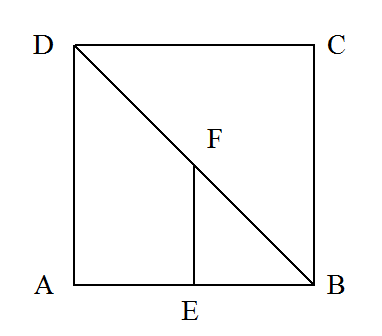
\includegraphics[width=5cm]{2ex1.png} 
\end{center}
\begin{qu} Dans le repère orthonormé (A ; B ; D), donner les coordonnées des points A, B, C, D, E et F. \end{qu}
\begin{qu} Dans le repère orthonormé (E ; B ; F), donner les coordonnées des points A, B, C, D, E et F.\end{qu}
\end{EX}

\begin{EX} \setcounter{ques}{0}
Cette figure est formée d’un carré, d’un rectangle et d’un triangle rectangle. 
\begin{center}
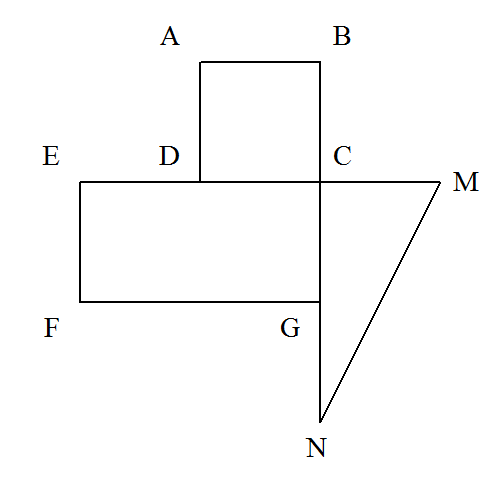
\includegraphics[width=5cm]{2ex2.png} 
\end{center}
\begin{qu} Donner les coordonnées de tous les points dans le repère orthonormé (C ; M ; B).\end{qu}
\begin{qu} Donner les coordonnées de tous les points dans le repère orthonormé (C ; D ; G).\end{qu}
\begin{qu} Donner les coordonnées de tous les points dans le repère orthonormé (E ; D ; F).\end{qu}
\begin{qu} Donner les coordonnées de tous les points dans le repère orthogonal (F ; G ; E).\end{qu}
\end{EX}

\begin{EX} \setcounter{ques}{0}
Dans un repère orthogonal \rIJ ~tel que $OI=1cm$ et $OJ=2cm$, placer les points suivants :
$$A(2\,;\,2) \qquad B(-1\,;\,1) \qquad C(-4\,;\,-2) \qquad D(5\,;\,1) \qquad E(3\,;\,0)$$
\end{EX}

\newpage \setcounter{ques}{0}
\noindent\begin{minipage}{.20\linewidth}\begin{center}                   % Lycée en haut à droite
\noindent \emph{Lycée Paul Lapie - Courbevoie}
\end{center}\end{minipage}
\begin{minipage}{1.5\linewidth}\begin{center}		% Classe  gauche
\noindent \cl\\ Chapitre 2
\end{center}\end{minipage}

\begin{center}\shadowbox{ \Large Planche d'exercices n°2(bis) : Repères, coordonnées, distance, milieu } 		% Titre du chapître
\end{center}

On se place dans un repère orthonormé \rIJ.

\begin{EX}
Dans chaque cas, donnez la nature du triangle ABC :
\begin{qu} ~~ $A(0\,;\,0)$, $B(1\,;\, -3)$, $C(3\,;\,-1)$.
\end{qu} \begin{qu} ~~ $E(2\,;\,1)$, $F(-1\,;\,1+\sqrt 3)$, $G( -1\,;\, 1-\sqrt 3)$.
\end{qu} \begin{qu} ~~ $M(-1 \,;\,-1)$, $N(1\,;\,3 )$, $P(5\,;\, 1)$. 
\end{qu}
\begin{qu} Calculez le périmètre du triangle EFG.
\end{qu}
\begin{qu} Calculez l'aire du triangle MNP.
\end{qu}

\end{EX}

\begin{EX}
Répondez Vrai ou Faux et justifiez les réponses.
\setcounter{ques}{0}
\begin{qu}
 Le quadrilatère OABC est un rectangle, avec $A(1\,;\,2)$, $B(5\,;\,0)$, $C(4\,;\,-2)$ et $O$ origine sur repère.
\end{qu} \begin{qu} Le point $M(-1\,;\,5)$ appartient à la médiatrice du segment [AB], avec $A(-4 \,;\,-1)$ et $B(5\,;\,2)$.
\end{qu} \begin{qu} Le point $F(-4\,;\,9)$ appartient au cercle de centre O et de rayon 10, avec $O$ origine sur repère.
\end{qu}
\end{EX}

\begin{EX}
On se donne les quatre points : $A(0\,;\,-2)$, $B(3\,;\,-1)$, $C(2\,;\,2)$ et $D(-1\,;\,1)$.

Quelle est la nature du quadrilatère ABCD ?
\end{EX}

\begin{EX}
Soit les points $A(3\,;\,2)$, $B(6,5\,;\,10)$, $C(-4,5\,;\,-2,5).$\\
Le point $C$ appartient-il au cercle de centre $A$, passant par $B$ ?
\end{EX}

\begin{EX}
On se donne les quatre points : $A(2\,;\,4)$, $B(-2\,;\,2)$, $C(-3\,;\,-1)$ et $D(5\,;\,-5)$.
\begin{qu} Démontrez que A, B, C, D appartiennent à un même cercle de centre $M(2\,;\,-1)$.
\end{qu}
\begin{qu} Calculez les longueurs des côtés et des diagonales du polygone $ABCD$.
\end{qu}
\begin{qu} Vérifiez que : $AB\x CD + BC \x AD = AC \x BD$.
\end{qu}
\begin{Sbox}\begin{minipage}{0.9\linewidth}
{\bf{ Point histoire :}} Ptolémée était un astronome, mathématicien et géographe grec du IIème siècle après JC. Il a démontré le théorème suivant : \\
Un quadrilatère convexe est inscriptible dans un cercle {\bf{si et seulement si}} le produit des diagonales est égal à la somme des produits des côtés opposés : 
\begin{center}
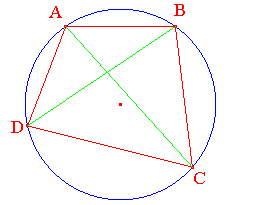
\includegraphics[width=5cm]{2ptolem.png} \quad\quad \quad \quad $AB\x CD + BC \x AD = AC \x BD$.
\end{center}
\end{minipage}\end{Sbox}\begin{center}\fbox{\TheSbox}\end{center}

\end{EX}

\newpage \setcounter{EXO}{0}
\noindent\begin{minipage}{.20\linewidth}\begin{center}                  
\noindent \emph{Lycée Paul Lapie - Courbevoie}
\end{center}\end{minipage}
\begin{minipage}{1.5\linewidth}\begin{center}	
\noindent \cl\\ Chapitre 2 (bis)
\end{center}\end{minipage}

\begin{center}\shadowbox{ \Large Planche n°2 (ter) : Configuration planes} 	
\end{center}

\begin{EX} Dans un repère orthonormé, on considère les points : $A(1\,;\,4) ~~ B(3\,;\,-2)~~C(9\,;\,1)$
 \begin{enumerate}
\item Faire une figure que l'on complètera au fur et à mesure.
\item Calculer les coordonnées de K milieu de $[AB]$
\item La parallèle à (BC) passant par K coupe (AC) en L. Calculer les coordonnées de L. Justifier.
\end{enumerate}

\end{EX}


\begin{EX}  Dans un repère orthonormé, on considère les points : $A(-2\,;\,5) ~~ B(4\,;\,3)~~C(8\,;\,-3)~~D(2\,;\,-1)$
 \begin{enumerate}
\item Calculer les coordonnées de K milieu de $[AC]$ et du milieu L de [BD].
\item Montrer que le quadrilatère ABCD est un parallélogramme.
\end{enumerate}
\end{EX}


\begin{EX}  Dans un repère orthonormé, on considère les points : $E(1\,;\,-1) ~~ F(5\,;\,3)~~C(3\,;\,1)~~H(2\,;\,3)$
 \begin{enumerate}
\item Démontrer que F est le symétrique de E par rapport à C.
\item Calculer les coordonnées du point K symétrique de H par rapport à C.
\item Donner la nature exacte du quadrilatère EKFH. Justifier.
\end{enumerate}
\end{EX}

\begin{EX} Dans un repère orthonormé, on considère les points : $A(1\,;\,1) ~~ B(5\,;\,2)~~C(3\,;\,4)$ \\
Calculer les coordonnées de D afin que ABCD soit un parallélogramme.

\end{EX}

\begin{EX}  Dans un repère orthonormé, on considère les points : $A(3\,;\,1) ~~ B(2\,;\,3)~~C(-4\,;\,0)~~D(-3\,;\,-2)$
 \begin{enumerate}
\item Calculer les coordonnées de M milieu de $[AC]$ et du milieu L de [BD].
\item Que peut-on en déduire sur la nature du quadrilatère ABCD ? Justifier.
\item Démontrer que le quadrilatère ABCD est un rectangle.
\item Est-ce un carré ? Justifier.
\end{enumerate}
\end{EX}


\begin{EX}  Dans un repère orthonormé, on considère les points : $M(-1\,;\,-1) ~~ N(1\,;\,3)~~P(5\,;\,1)~~Q(3\,;\,-3)$ \\
Démontrer que le quadrilatère MNPQ est un carré.
\end{EX}




\newpage \setcounter{EXO}{0}


\noindent\begin{minipage}{.20\linewidth}\begin{center}                  
\noindent \emph{Lycée Paul Lapie - Courbevoie}
\end{center}\end{minipage}
\begin{minipage}{1.5\linewidth}\begin{center}	
\noindent \cl\\ Chapitre 3
\end{center}\end{minipage}

\begin{center}\shadowbox{ \Large Planche n° 3 : Généralités sur les fonctions } 	
\end{center}


\begin{EX}
\begin{qu} $f$ est la fonction définie sur \R par $f(x)=\f{1}{x^2+2}$. Calculer les images par $f$ des réels $-2$ ; $0$ ; $1$ ; $\sqrt{2}$.
\end{qu}
\begin{qu} $g$ est la fonction définie sur \R par $g(x)=x^2+x-5$. Calculer les images par $g$ des réels $4$ ; $6$ ; $-5$ ; $0$.
\end{qu}
\end{EX}

\begin{EX}
$f$ est une fonctions et $\mathcal{C}_f$ sa représentation graphique. Traduire par des égalités du type $y=f(x)$ chacune des phrases suivantes :
\begin{qu} $\mathcal{C}_f$ passe par le point $(-2\,;\,5)$.
\end{qu}
\begin{qu} $\mathcal{C}_f$ coupe l'axe des ordonnées au point d'ordonnée $-1$.
\end{qu}
\begin{qu} $\mathcal{C}_f$ coupe l'axe des abscisses aux points d'abscisses respectives $-2$ et $3$.
\end{qu}
\end{EX}

\begin{EX}
Pour chaque fonction, calculer le ou les antécédents de $a$ par $f$ :
\begin{qu} $f(x)=2x-7$ \qquad $a=5$
\end{qu}
\begin{qu} $f(x)=3x-4$ \qquad $a=2$
\end{qu}
\begin{qu} $f(x)=x^2-4x$ \qquad $a=-4$
\end{qu}
\begin{qu} $f(x)=x^2$ \qquad $a=9$
\end{qu}
\begin{qu} $f(x)=(x-4)(2x+6)$ \qquad $a=0$
\end{qu}
\begin{qu} $f(x)=49x^2-28x$ \qquad $a=-4$
\end{qu}

\end{EX}

\begin{EX}
Parmi les courbes suivantes, retrouver la courbe représentative de la fonction $f$, sachant que :
\begin{itemize}
\item 1 a pour image 0 par $f$,
\item 0 a pour image 2 par $f$,
\item 5 est l'image de $3$ et $5$ par $f$,
\item si $x\in [3\,;\,5]$ alors $f(x) \se 5$,
\item l'équation $f(x)=0$ a deux solutions.
\end{itemize}
\begin{center}
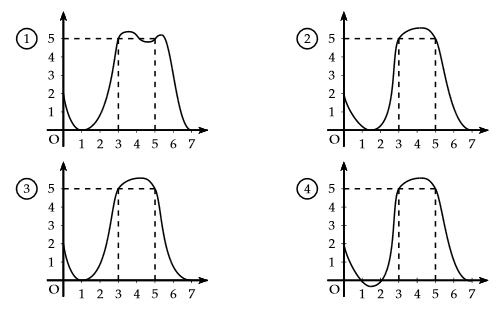
\includegraphics[width=12cm]{3ex1.png}
\end{center}
\end{EX}






\newpage \setcounter{EXO}{0}


\noindent\begin{minipage}{.20\linewidth}\begin{center}                  
\noindent \emph{Lycée Paul Lapie - Courbevoie}
\end{center}\end{minipage}
\begin{minipage}{1.5\linewidth}\begin{center}	
\noindent \cl\\ Chapitre 5
\end{center}\end{minipage}

\begin{center}\shadowbox{ \Large Planche n°5  : Information Chiffrée } 	
\end{center}
\medskip
\begin{EX} Une entreprise commercialise $10,7$ millions de voitures par an. Parmi tous les modèles vendus, $\np{1605000}$ voitures sont électriques.
\begin{enumerate}
\item Quelles sont ici la population et la sous-population étudiées ? 
\item Quel pourcentage de la population totale représentent les voitures électriques ?
\end{enumerate}
\end{EX}
\begin{EX}Dans une population d'insectes, on dénombre $\np{2000}$ insectes porteurs d'un gène destructeur pour la population humaine. Ces insectes destructeurs représentent $1,5\%$ de la population totale des insectes. \\
Quel est le nombre d'insectes dans cette population ?
\end{EX}
\begin{EX} On estime la population mondiale au 1er janvier 2020 à $\np{7 794 799}$ milliers d'habitants, et celle de l'Europe à $\np{745216}$ milliers d'habitants.
\begin{enumerate}
\item Quelle proportion de la population mondiale représente la population de l'Europe selon ces estimations en 2020?
\item Sachant que l'Europe de l'Ouest compterait $\np{196146}$ milliers d'habitants, quelle proportion de la population européenne cela représenterait-il ?
\item Calculer de deux manières différentes la proportion de la population mondiale habitant en Europe de l'Ouest ?
\end{enumerate}
\end{EX}
\begin{EX} Le prix d'un article valant initialement $120$\EUR a baissé de $30\%$ durant les soldes. 
\begin{enumerate}
\item Quel est le montant de la remise ?
\item Quel est le nouveau prix de cet article ?
\item Comment pouvait-on calculer directement le nouveau prix sans calculer la remise ?
\end{enumerate}
\end{EX}

\begin{EX} Une entreprise compte 250 salariés en 2018. Suite à une augmentation des commandes, elle embauche 35 personnes en 2019. 
\begin{enumerate}
\item Que représente le nombre 35 ?
\item Quel est le nombre de salariés dans l'entreprise après le recrutement ?
\item Quel pourcentage représentent les embauches par rapport à l'effectif des salariés de 2018 ?
\item En 2020, l'entreprise embauche encore 12 salariés. Quel est le taux d'augmentation du nombre de salariés entre 2018 et 2020 ?
\end{enumerate}
\end{EX}

\begin{EX} 
Deux offres sont proposées sur une bouteille de lessive. 
\begin{center}
\og 15\% de produit en plus \fg{} \hspace{2cm} \og Baisse de 15\% du prix \fg{} 
\end{center}
Quelle offre est la plus avantageuse ?
\end{EX}

\begin{EX} Lundi, Audrey possède une certaine somme d'argent $S$ dans sa tirelire. Mardi, elle ajoute $40\%$ de cette somme. Mercredi, elle ajoute $30 \%$ de la nouvelle somme dans sa tirelire. Puis jeudi, elle ajoute $20\%$ de la nouvelle somme. Enfin, vendredi, elle ajoute $10\%$ du total de sa tirelire. Le samedi, elle décide de dépenser tout ce qu'elle a ajouté cette semaine, et sa tirelire dispose à nouveau de la somme de départ $S$. 
\begin{enumerate}
\item Quel a été le taux global d'évolution de la somme S entre lundi et vendredi ?
\item Quel a été le taux réciproque le samedi ? Arrondir à $0.1\%$ près.
\end{enumerate}
\end{EX}





\newpage \setcounter{EXO}{0}

\noindent\begin{minipage}{.20\linewidth}\begin{center}                  
\noindent \emph{Lycée Paul Lapie - Courbevoie}
\end{center}\end{minipage}
\begin{minipage}{1.5\linewidth}\begin{center}	
\noindent \cl \\ Chapitre 6
\end{center}\end{minipage}

\begin{center}\shadowbox{ \Large Planche n°  6  : \'Etude qualitative de fonctions } 	
\end{center}

\begin{EX}
Voici la courbe représentative de la fonction $f$. Donner \df ~et tracer son tableau de variation. \\
\begin{center} 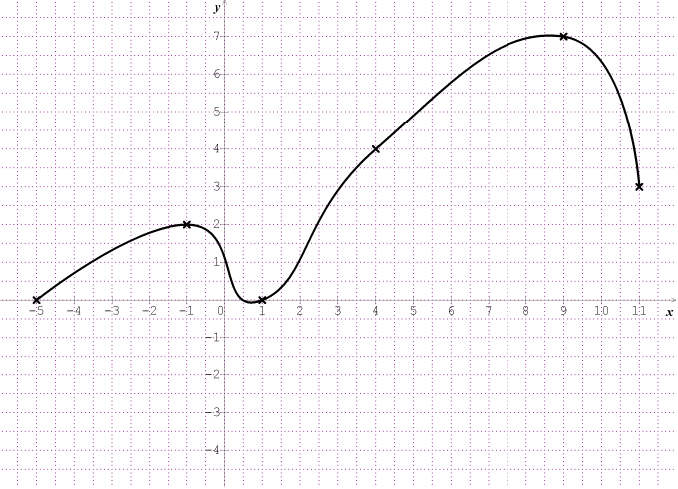
\includegraphics[width=10cm]{6ex1.png}
\end{center}
\end{EX}
\begin{EX}
 Soit la fonction $f$ dont le tableau de variations est donné ci-dessous. 

\begin{center}\begin{variations}
   x       &\quad -8 &  & -2 &   & 1 &   & 5 & & 7 \quad\\
   \filet
   \m{f}&\quad \h 4\, & \d & -1 \,& \c & \h 0 \, & \d  & -2 & \c & \h{-1} \quad \\
 \end{variations} \end{center}
\begin{qu} Donner \df~ . \end{qu}
\begin{qu} Tracer une courbe représentative de $f$ compatible avec ce tableau de variation.\end{qu}
\begin{qu} Quel est le maximum de $f$ sur son ensemble de défnition ?\end{qu}
\begin{qu} Quel est le mimimum de $f$ sur son ensemble de défnition ?\end{qu}
\begin{qu} Quel est le maximum de $f$ sur $[1\,;\,7]$ ? \end{qu}
\begin{qu} Quel est le minimum de $f$ sur $[-2\,;\,5]$ ? \end{qu}
\end{EX}

\begin{EX}
Tracer la courbe représentative d'une fonction $f$ telle que :
\begin{itemize}
\item $f$ est définie sur \R ,
\item $f$ est croissante sur $] - \infty \,;\, -1 ]$, puis sur $ [3 \,;\, + \infty[$, 
\item $f$ est décroissante sur $[-1\,;\,3]$,
\item le maximum de $f$ sur \R~est 3, atteint pour $x=-1$,
\item le minimum de $f$ sur \R~est -4, atteint pour $x=3$,
\item lorsque $x$ se rapproche de $-\infty$, $f(x)$ se rapproche de 0,
\item lorsque $x$ se rapproche de $+\infty$, $f(x)$ se rapproche de -1. \end{itemize}

\end{EX}
\newpage \setcounter{EXO}{0}
\noindent\begin{minipage}{.20\linewidth}\begin{center}                  
\noindent \emph{Lycée Paul Lapie - Courbevoie}
\end{center}\end{minipage}
\begin{minipage}{1.5\linewidth}\begin{center}	
\noindent \cl \\ Chapitre 6
\end{center}\end{minipage}

\begin{center}\shadowbox{ \Large Planche n°  6 (bis) : \'Etude qualitative de fonctions } 	
\end{center}

\begin{EX}
$f$ est une fonction définie sur \R. Résoudre graphiquement les inéquations suivantes : 
$$f(x) > 3 \hspace{3cm} f(x) \ie -3$$
\begin{center}
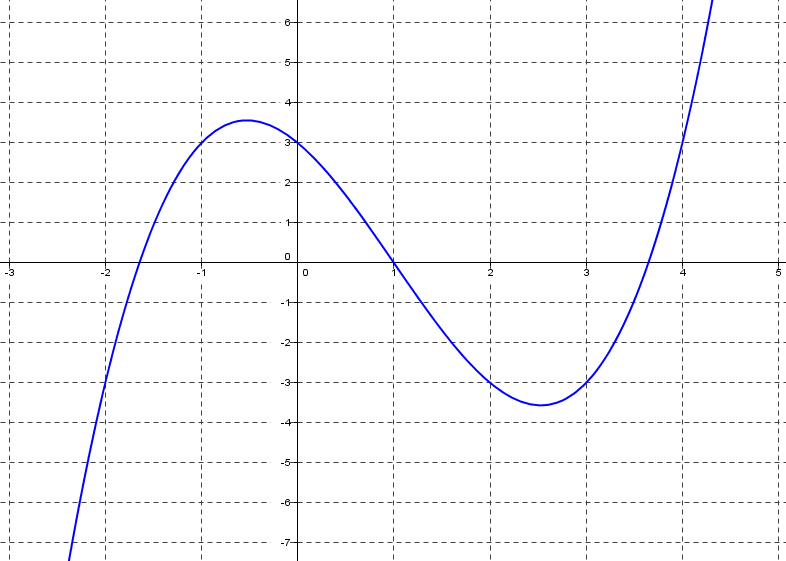
\includegraphics[width=13cm]{6ine.png}
\end{center}
\end{EX}

\begin{EX}
$f$ et $g$ sont deux fonctions définies sur \R. Résoudre graphiquement l'inéquation suivante : 
$$f(x) < g(x) $$
\begin{center}
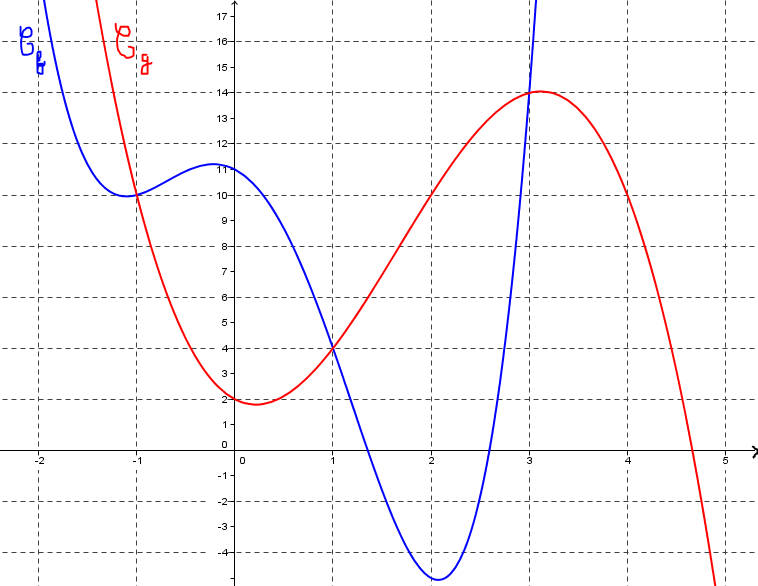
\includegraphics[width=13cm]{6inters.png}
\end{center}
\end{EX}
\newpage \setcounter{EXO}{0}
\noindent\begin{minipage}{.20\linewidth}\begin{center}                  
\noindent \emph{Lycée Paul Lapie - Courbevoie}
\end{center}\end{minipage}
\begin{minipage}{1.5\linewidth}\begin{center}	
\noindent \cl \\ Chapitre 6
\end{center}\end{minipage}

\begin{center}\shadowbox{ \Large Planche n° 6 (ter) : \'Etude qualitative de fonctions } 	
\end{center}

\begin{EX}
$f$ est une fonction définie sur $[-5\,;\,14]$. Résoudre graphiquement les inéquations suivantes : 
$$(a.)~~f(x) < 1 \hspace{3cm} (b.)~~f(x) \se -3$$
\begin{center}
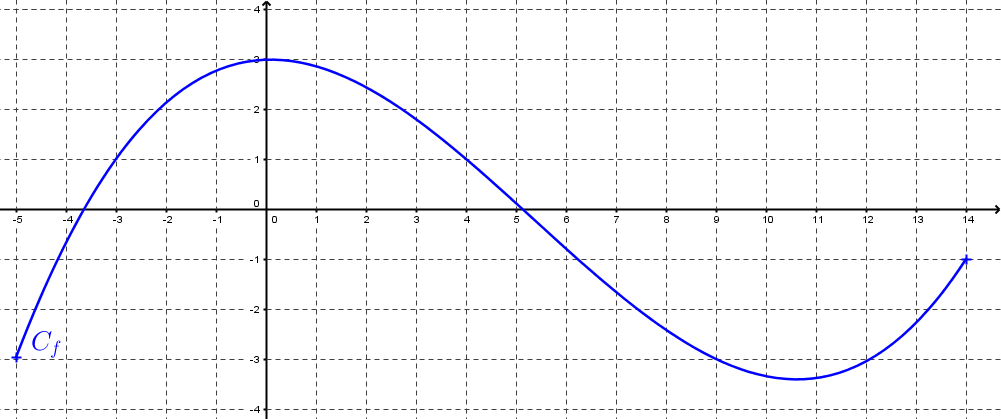
\includegraphics[width=15cm]{6exo1.png}
\end{center}
\end{EX}

\begin{EX} $g$ est fonction définie sur $[-3 \,;\, 5]$, dont le tableau de variations est donné ci-dessous :
\begin{center}\begin{variations}
   x       &\quad -3 &  & -2 &   & 0 &   & 5 \quad\\
   \filet
   \m{g}&\quad \h 0\, & \d & -4 \,& \c & \h {2,5} \, & \d  & -1 \quad \\
 \end{variations}\end{center}

Complétez les écritures suivantes avec \og $<$ \fg ~,~\og $>$ \fg ~,~\og $=$ \fg ~ou~\og on ne sait pas \fg.
$$g(-1) \hspace{0.8cm} g(-2) \hspace{5cm} g(4,5) \hspace{0.8cm} g(3) $$  $$ g(-2,5) \hspace{0.8cm} 0 \hspace{5.6cm} g(-1) \hspace{0.8cm} 2,5 $$
$$ g(-1) \hspace{0.8cm} g(1) \hspace{5.4cm} g(0) \hspace{0.8cm} -3 $$
$$ g(-3) \hspace{0.8cm} 0 \hspace{6cm} -1 \hspace{0.8cm} g(1) $$
\end{EX}





\newpage \setcounter{EXO}{0}

\noindent\begin{minipage}{.20\linewidth}\begin{center}                   
\noindent \emph{Lycée Paul Lapie - Courbevoie}
\end{center}\end{minipage}
\begin{minipage}{1.5\linewidth}\begin{center}		
\noindent \cl\\ Chapitre 7
\end{center}\end{minipage}

\begin{center}\shadowbox{\Large Planche n° 7 : Fonction affines } 	
\end{center}

\begin{EX}
Faire la représentation graphique des fonctions suivantes :
\begin{center}\begin{tabular}{p{4cm} p{4cm}p{4cm}p{4cm}}
\textbf{a.~~} $f(x)=-x+2$&\textbf{b.~~} $g(x)=\displaystyle{\frac{1}{2}}x-1$&\textbf{c.~~}$h(x)=2.5x-3 $&\textbf{d.~~}$k(x)=-2x+4$\\
\end{tabular}\end{center}
\end{EX}
\begin{EX}
Donner le tableau de signes des fonctions suivantes :
$$f(x)=(3-x)(2x+8) \hspace{2cm} g(x)=\f{x-1}{3x+9} \hspace{2cm} h(x)=\f{(5-x)(2x-1)}{(x-3)(4x+2)}$$
\end{EX}
\begin{EX}
Lire graphiquement pour chaque droite ci-dessous les valeurs des coefficients directeurs et des ordonnées à l'origine :
\begin{center}
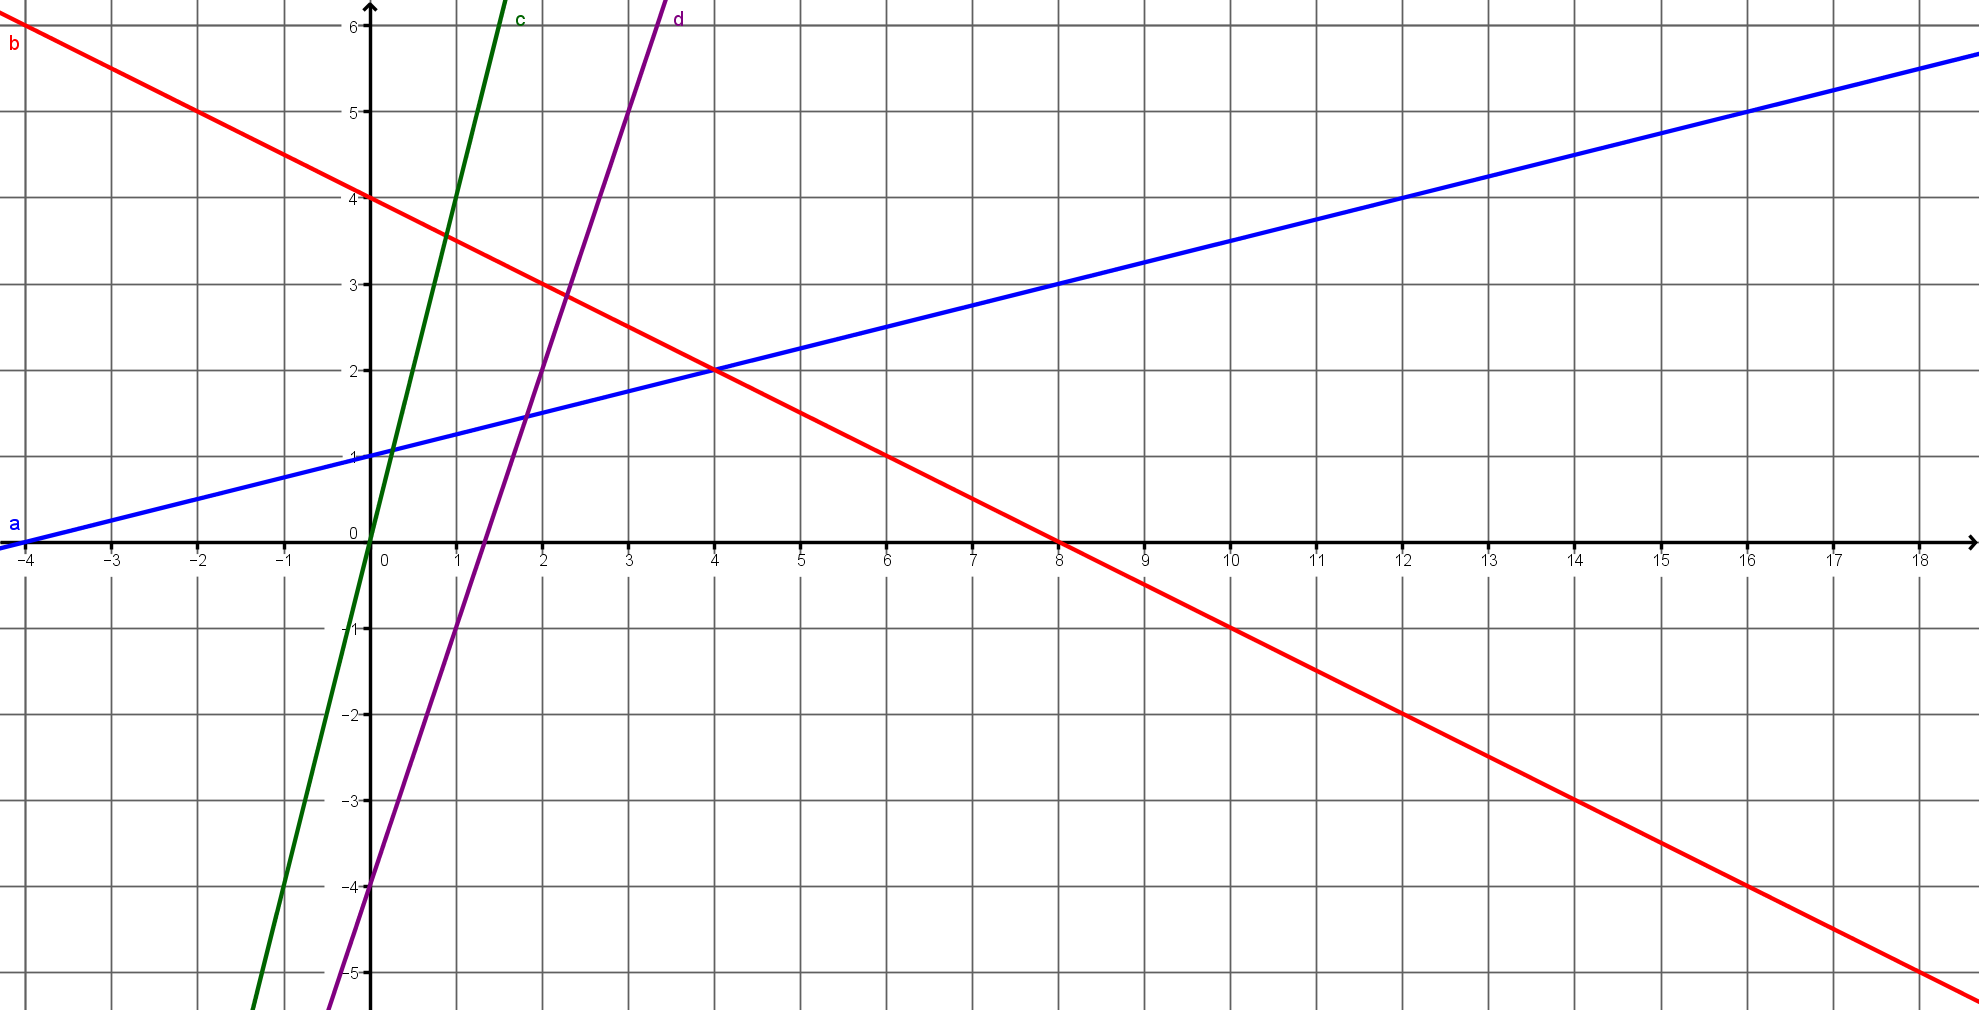
\includegraphics[width=15cm]{7exo.png}
\end{center}
\end{EX}
\begin{EX}
On considère la droite (MN), dans chaque cas, calculez la valeur du coefficient directeur et de l'ordonnée à l'origine de la fonction affine associée:
\begin{center}\begin{tabular}{p{4cm} p{4cm}p{4cm}p{4cm}}
\textbf{a.~~}  $ M(-2\,;\,1) ~~,~~  N(3\,;\,9). $&\textbf{b.~~}$ M(\f{1}{2} \,;\,1)~~,~~ N(1\,;\, \f{4}{5}). $&\textbf{c.~~}$ M(-2 \,;\,3)~~,~~ N(5 \,;\,-4). $&\textbf{d.~~}$ M(4 \,;\,-7)~~,~~ N(-2 \,;\,-2). $\\
\end{tabular}\end{center}\end{EX}

\begin{EX}
Résoudre par le calcul les équations et inéquations suivantes :
\begin{center}\begin{tabular}{p{4cm} p{4cm}p{4cm}p{4cm}}
\textbf{a.~~} $6x-4=3x+5$&\textbf{b.~~}$-8x+12<4x-13$&\textbf{c.~~}$-14x-3>11x-12$&\textbf{d.~~}$2x-6>-x+2$\\
\end{tabular}\end{center}
\end{EX}
\begin{EX} Les spectateurs d'une course de motocross ont garé leurs véhicules (voiture ou moto) sur un parking. On y compte à présent 65 véhicules, pour un total de 180 roues. Combien y at-il de motos sur le parking ? \\
\emph{On résoudra ce problème à l'aide d'une équation du premier degré.}
\end{EX}
{\bf{Exercices du livre : chapitre 3 : n° 9, 16, 18, 19, 21, 36, 38, 41, 42.}}

\newpage \setcounter{EXO}{0}

\noindent\begin{minipage}{.20\linewidth}\begin{center}                   
\noindent \emph{Lycée Paul Lapie - Courbevoie}
\end{center}\end{minipage}
\begin{minipage}{1.5\linewidth}\begin{center}		
\noindent \cl\\ Chapitre 7
\end{center}\end{minipage}

\begin{center}\shadowbox{\Large Planche n° 7(bis) : Fonctions affines} 	
\end{center}

\begin{EX}
On suppose que l'accroissement de hauteur d'eau dans une citerne est proportionnel au temps écoulé.
\begin{enumerate}
\item Sachant que la hauteur d'eau est de 1m à l'instant $t=0$, et qu'elle augmente de $14cm$ toutes les 30 minutes, à quel moment cette hauteur est-elle égale à $2m$ ?
\item Tracer dans un repère la courbe qui donne la hauteur d'eau en fonction du temps.
\end{enumerate}
\end{EX}


\begin{EX} Lors de l'ouverture d'une nouvelle enseigne, les clients sont informés de l'offre suivante :
\begin{itemize}
\item si le prix affiché est inférieur ou égal à $100$ \EUR, le montant facturé est égal au prix affiché.
\item  si le prix affiché est strictement supérieur à $100$ \EUR, et inférieur ou égal à $200$ \EUR, le montant facturé est égal au prix affiché diminué de 5\%.
\item  si le prix affiché est strictement supérieur à $200$ \EUR, le montant facturé est égal au prix affiché diminué de 10\%.
\end{itemize}
On note $f$ la fonction définie sur l'intervalle $[0\,;\,250]$ qui, à un prix affiché, fait correspondre le prix facturé.\\
Tracer dans un repère la représentation graphique de la fonction $f$.
\end{EX}


\begin{EX}
Un installateur en appareils électroménagers fait payer à ses clients $40$\EUR ~de frais de déplacements et $30$\EUR ~par heure de travail.
\begin{enumerate}
\item Quel est le montant de la facture pour $2$h de travail ? \'Ecrire le montant $D(x)$ de la facture en fonction du nombre $x$ d'heures de travail.
\item Représenter graphiquement la fonction $D$.
\item Lire sur le graphique le montant de la facture pour $2h30$ de travail, pour $4h$ de travail et puis pour $5h30$ de travail. Retrouver ces résultats par le calcul.
\item Lire sur le graphique quel temps de travail correspond à une facture de $55$\EUR, puis à une facture de $85$\EUR. Retrouver ces résultats par le calcul. 
\end{enumerate} 
\end{EX}


\begin{EX} Un particulier souhait louer une voiture. L'agence de location $A$ demande $100$\EUR~au départ et $0,20$\EUR~par km. L'agence $B$ demande $150$\EUR ~au départ puis $0,15$\EUR ~par km. 

Donner, en fonction du nombre de km parcourus, l'agence qui sera la plus avantageuse.
\end{EX}

\begin{EX}
Diophante est un des grands savants de l'Antiquité. Il est le père de l'arithmétique moderne. Les équations « diophantiennes » forment un domaine à part entière des mathématiques. On ne sait que peu de choses de sa vie, mais l'énigme suivante a été élaborée par un de ses proches après sa mort :
\begin{itemize}
\item L'enfance de Diophante dura le sixième de sa vie.
\item La barbe lui crût après un douzième de plus.
\item Après encore un septième, il se maria.
\item Et il eut un fils cinq ans plus tard.
\item Le fils vécut moitié moins longtemps que son père.
\item Et Diophante mourut quatre ans après son fils.\end{itemize}
Combien d’années Diophante a-t-il vécu ? Justifier
\end{EX}

\begin{EX}
ABC est un triangle tel que BC=5 cm.
Soit $x$ un réel de l'intervalle [0;5], et soit F le point de $[BC]$ tel que $BF=x$ cm.
On note  $\mathcal{A}_{AFB}$ et $\mathcal{A}_{AFC}$ les aires respectives des triangles AFB et AFC.

\begin{enumerate}
\item  Pour quelle(s) valeur(s) de $x$ a-t-on $\mathcal{A}_{AFB}=\mathcal{A}_{AFC}$ ?
\item Pour quelle(s) valeur(s) de $x$ a-t-on $\mathcal{A}_{AFB}=\f{1}{2}\mathcal{A}_{AFC}$ ? 
\item Pour chacune des deux questions, justifier la réponse par un raisonnement faisant intervenir la résolution d'une équation d'inconnue $x$.
\end{enumerate}

\end{EX}
{\bf{Exercices du livre : chapitre 2 : n°30, 33, 44, 50, 53, 59, 63, 64.}}





\newpage \setcounter{EXO}{0}



\noindent\begin{minipage}{.20\linewidth}\begin{center}                  
\noindent \emph{Lycée Paul Lapie - Courbevoie}
\end{center}\end{minipage}
\begin{minipage}{1.5\linewidth}\begin{center}	
\noindent \cl\\ Chapitre 8
\end{center}\end{minipage}

\begin{center}\shadowbox{ \Large Planche n° 8 : Vecteurs et translation } 	
\end{center}

\begin{EX} 
ABC est un triangle. 
\begin{center}
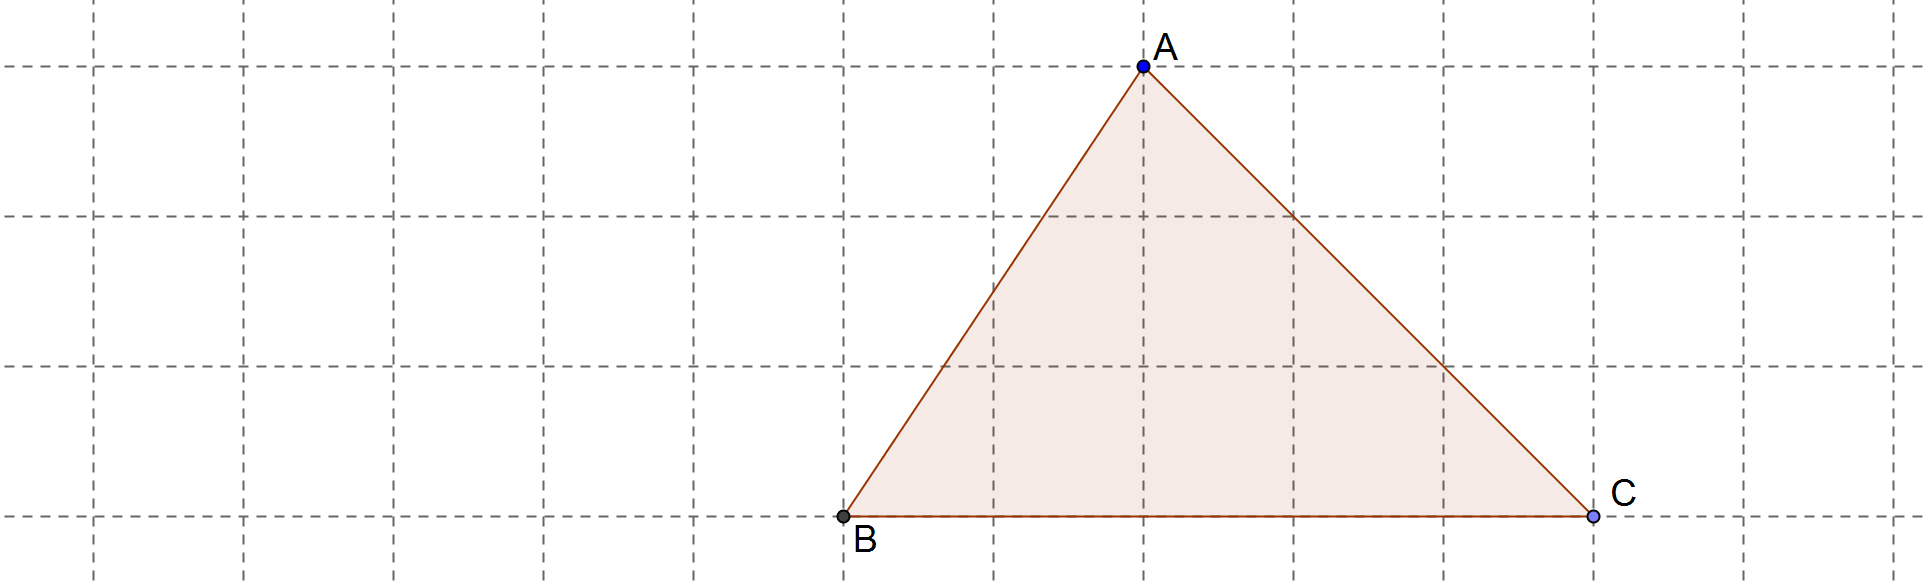
\includegraphics[width=11cm]{8ex1.png}
\end{center}
\begin{enumerate}
\item Placez le point I tel que $\v{CI}=\v{BA} $
\item Placez le point J tel que $\v{BJ}$ et $\v{BC}$ soient opposés.
\item Démontrez que JBIA est un parallélogramme.
\end{enumerate} 
\end{EX}

\begin{EX} 
\renewcommand{\tabularxcolumn}[1]{b{#1}}
\begin{tabularx}{\linewidth}{Xc}	
Sur la figure ci-contre, donnez deux vecteurs :

\begin{enumerate}
\item de même direction et de même sens mais qui ne sont pas égaux.
\item de même longueur qui ne sont pas égaux.
\item de même direction, de sens contraire, qui ne sont pas opposés.
\end{enumerate}
&
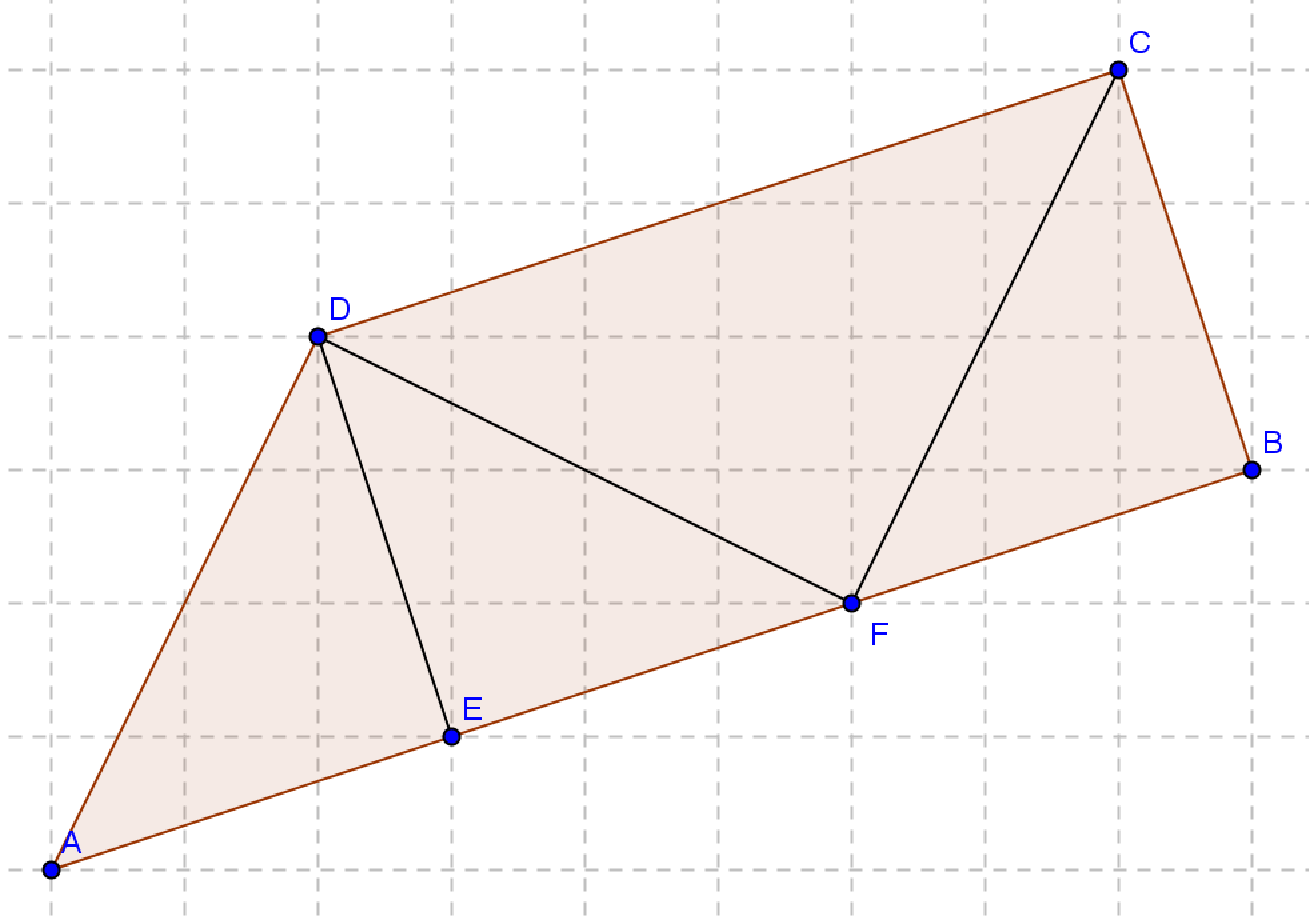
\includegraphics[width=7cm]{8ex2.png} \\
\end{tabularx}

\end{EX}

\begin{EX} 
ABC est un triangle quelconque.
\begin{enumerate}
\item  Construisez un point D tel que $\v{BD} = \v{AC}$ , puis le point J tel que A soit le milieu de [BJ].
\item Quelle est la nature du quadrilatère DCJA ?
\end{enumerate}
\end{EX}

\begin{EX} 
A, B, O et O’ sont quatre points distincts. 

C et D sont les symétriques respectifs de A et B par rapport à O. 

E et F sont les symétriques respectifs de A et B par rapport à O’.
~~~\\
Faites la figure puis démontrez que DCEF est un parallélogramme. 
\end{EX}

\begin{EX} 
Sur la figure ci-dessous, ABCD, ABDE, et ACDF sont des parallélogrammes. \\
Démontrez que ADEF en est un également.
\begin{center}
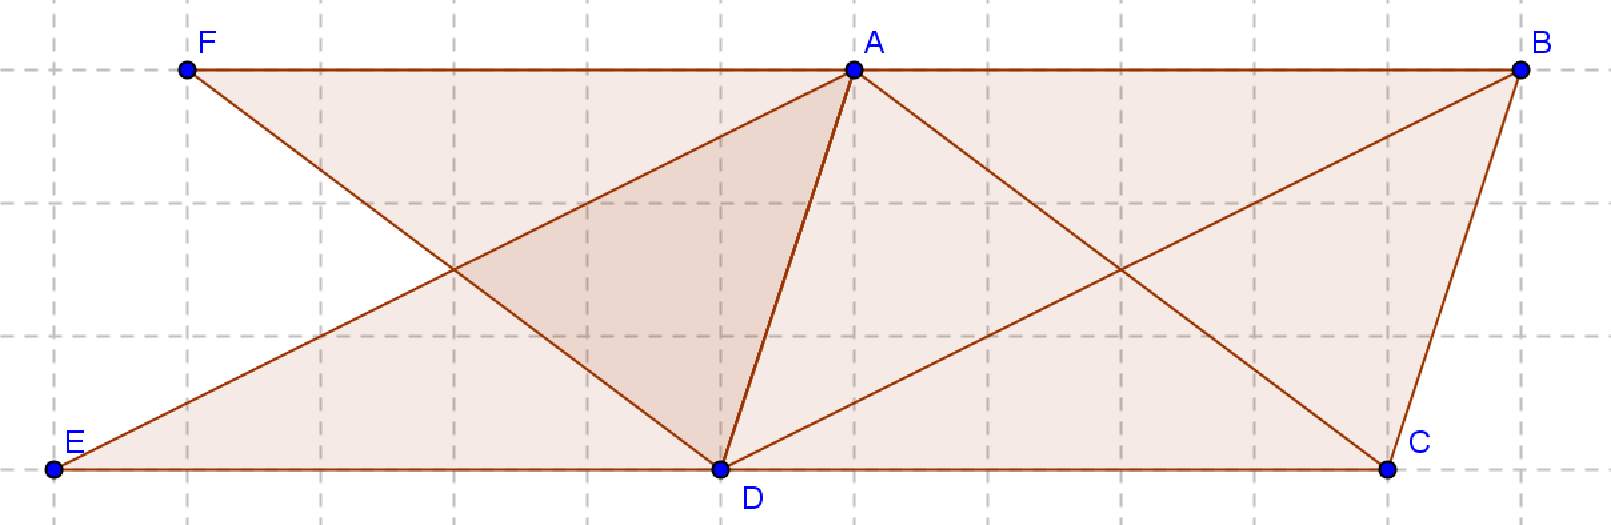
\includegraphics[width=10cm]{8ex5.png}
\end{center}\end{EX}

\begin{EX} 
ABCD est un parallélogramme.
\begin{center}
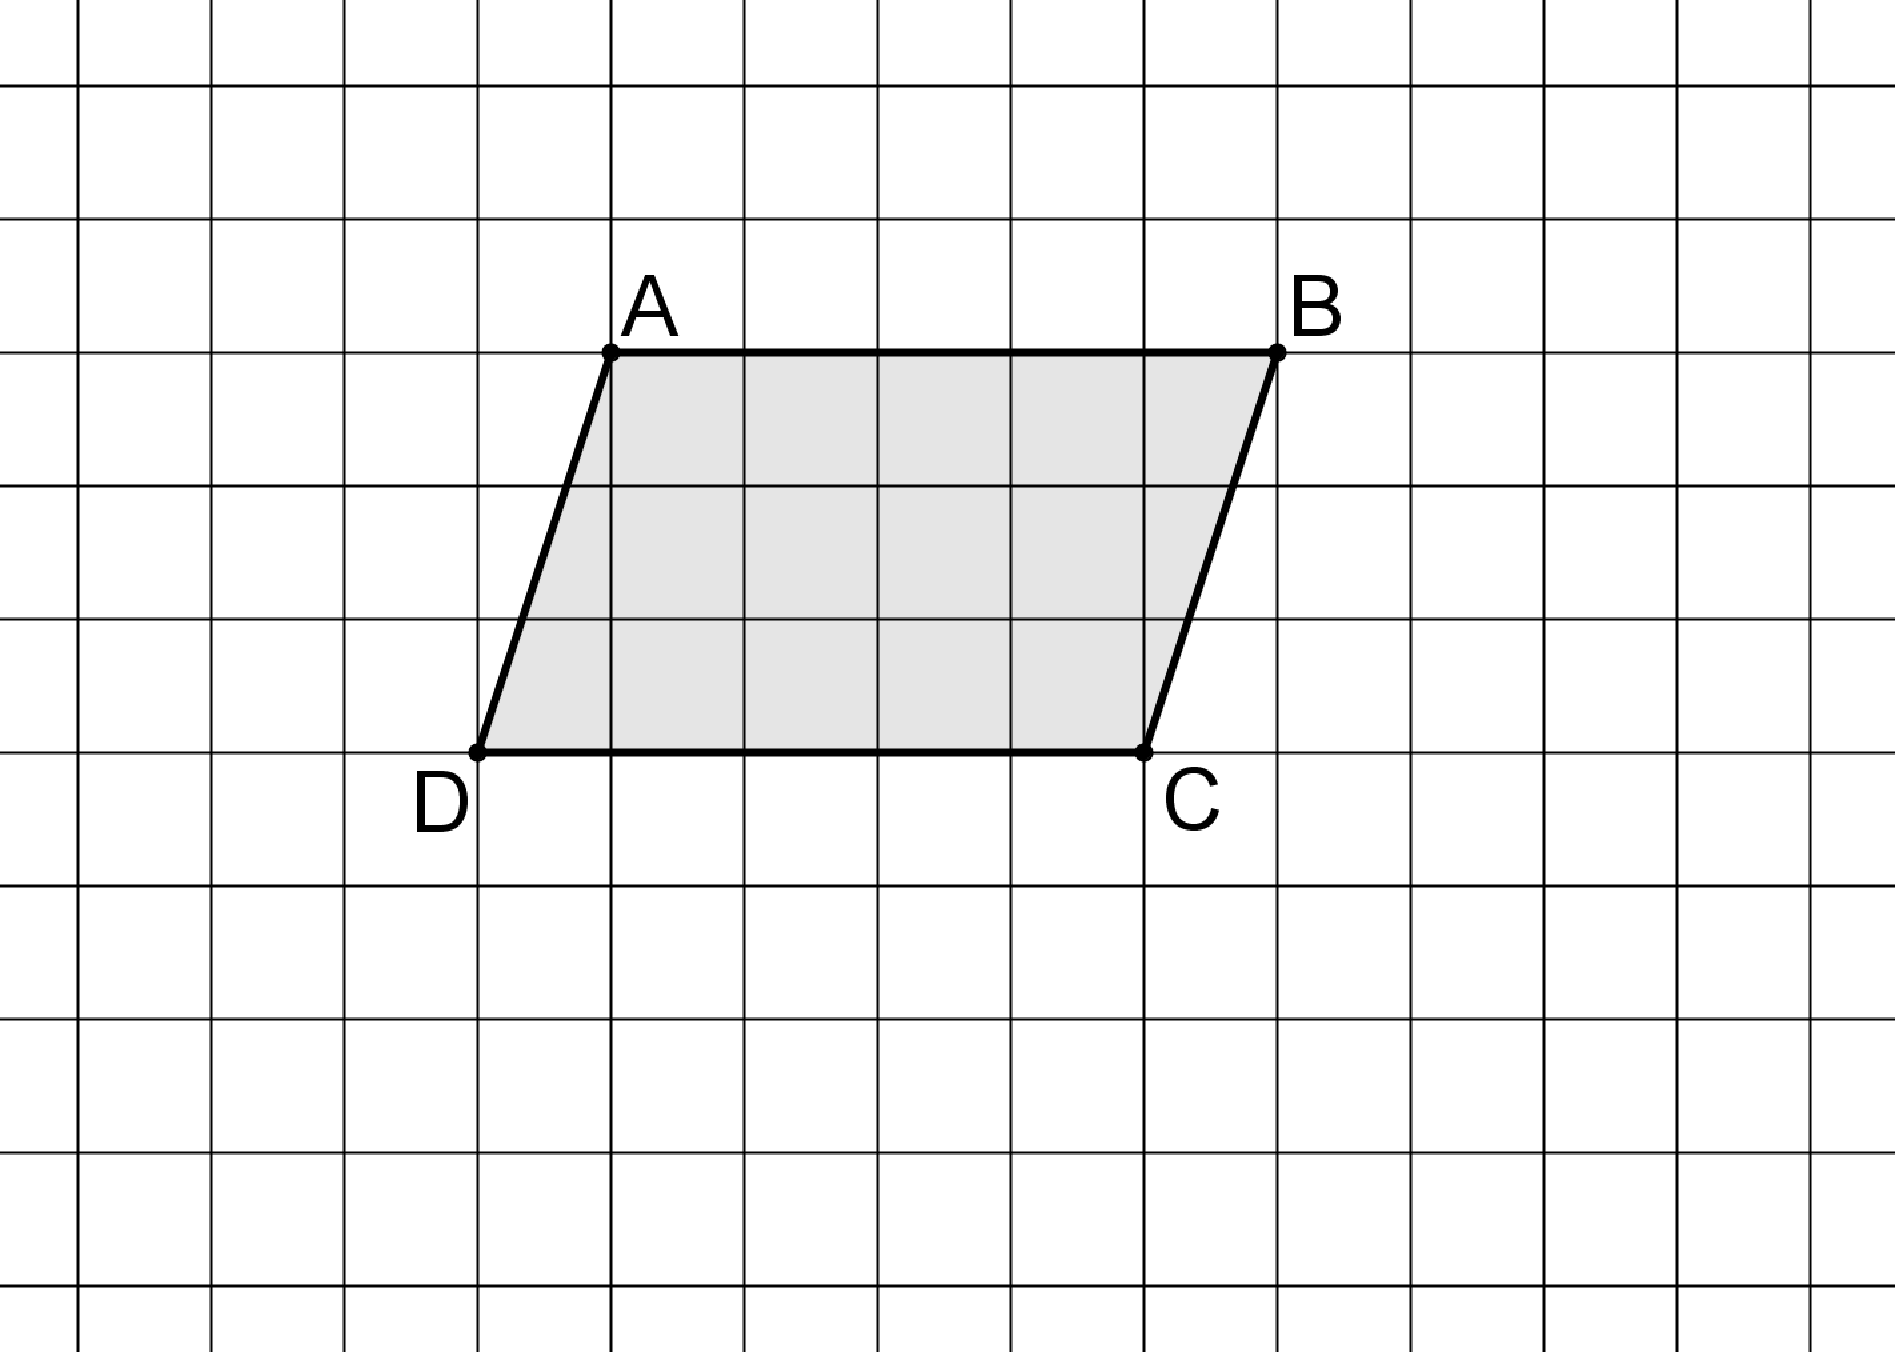
\includegraphics[width=8cm]{8ex6.png}
\end{center}
\begin{enumerate}
\item  Construire sur la figure ci-contre le point E tel que $\v{DE}=\v{AC}$.
\item Construire le point F, image de E par la translation de vecteur $\v{AB}$.
\item Quelle est la nature du quadrilatère DCFE ? Justifiez toutes les étapes de la démonstration.\end{enumerate}

\end{EX}

\begin{EX} 
Soit ABCD un rectangle de centre O.
\begin{enumerate}
\item  Représenter les transformés respectifs des points A, B, O, par la translation de vecteur $\v{AB}$.
\item Représenter les transformés respectifs des points A, B, O, par la translation de vecteur $\v{AD}$.
\item Représenter les transformés respectifs des points A, B, O, par la translation de vecteur $\v{OC}$.
\end{enumerate}
\end{EX}

\begin{EX} 
Pour chaque affirmation, dire si elle est vraie ou fausse en justifiant votre réponse :
\begin{enumerate}
\item  ABCD est un parallélogramme, donc $\v{AB}=\v{CD}$.
\item Une translation transforme E en F et G en H donc $[EH]$ et $[GH]$ ont même milieu.
\item ABCD et ABFE sont deux parallélogrammes, donc CDFE est un parallélogramme.
\item MATH est un parallélogramme, donc T est l'image de  H par la translation de vecteur $\v{MA}$.
\end{enumerate}
\end{EX}

\begin{EX} 

\vspace{0.3cm}

\renewcommand{\tabularxcolumn}[1]{b{#1}}
\begin{tabularx}{\linewidth}{Xc}	
On considère deux points A et B du plan. 

\vspace{0.3cm}

Construire le point I tel que $\v{AI}=\v{IB}$. 

\vspace{0.3cm}

Que pouvez-vous déduire du point I pour le segment $[AB]$ ?

&
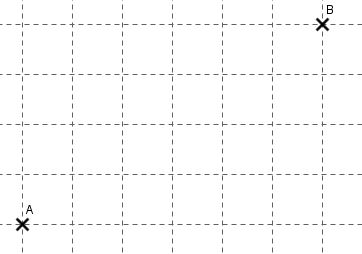
\includegraphics[width=6cm]{8ex9.png} \\
\end{tabularx}

\end{EX}


\newpage
\setcounter{EXO}{0}

\noindent\begin{minipage}{.20\linewidth}\begin{center}                  
\noindent \emph{Lycée Paul Lapie - Courbevoie}
\end{center}\end{minipage}
\begin{minipage}{1.5\linewidth}\begin{center}	
\noindent \cl\\ Chapitre 8
\end{center}\end{minipage}

\begin{center}\shadowbox{ \Large Planche n° 8 (bis) : Vecteurs et colinéarité} 	
\end{center}

\begin{EX}  On considère deux points A et B du plan ci-dessous, et trois vecteurs $\v{u}$ $\v{v}$ $\v{w}$.
\begin{center}
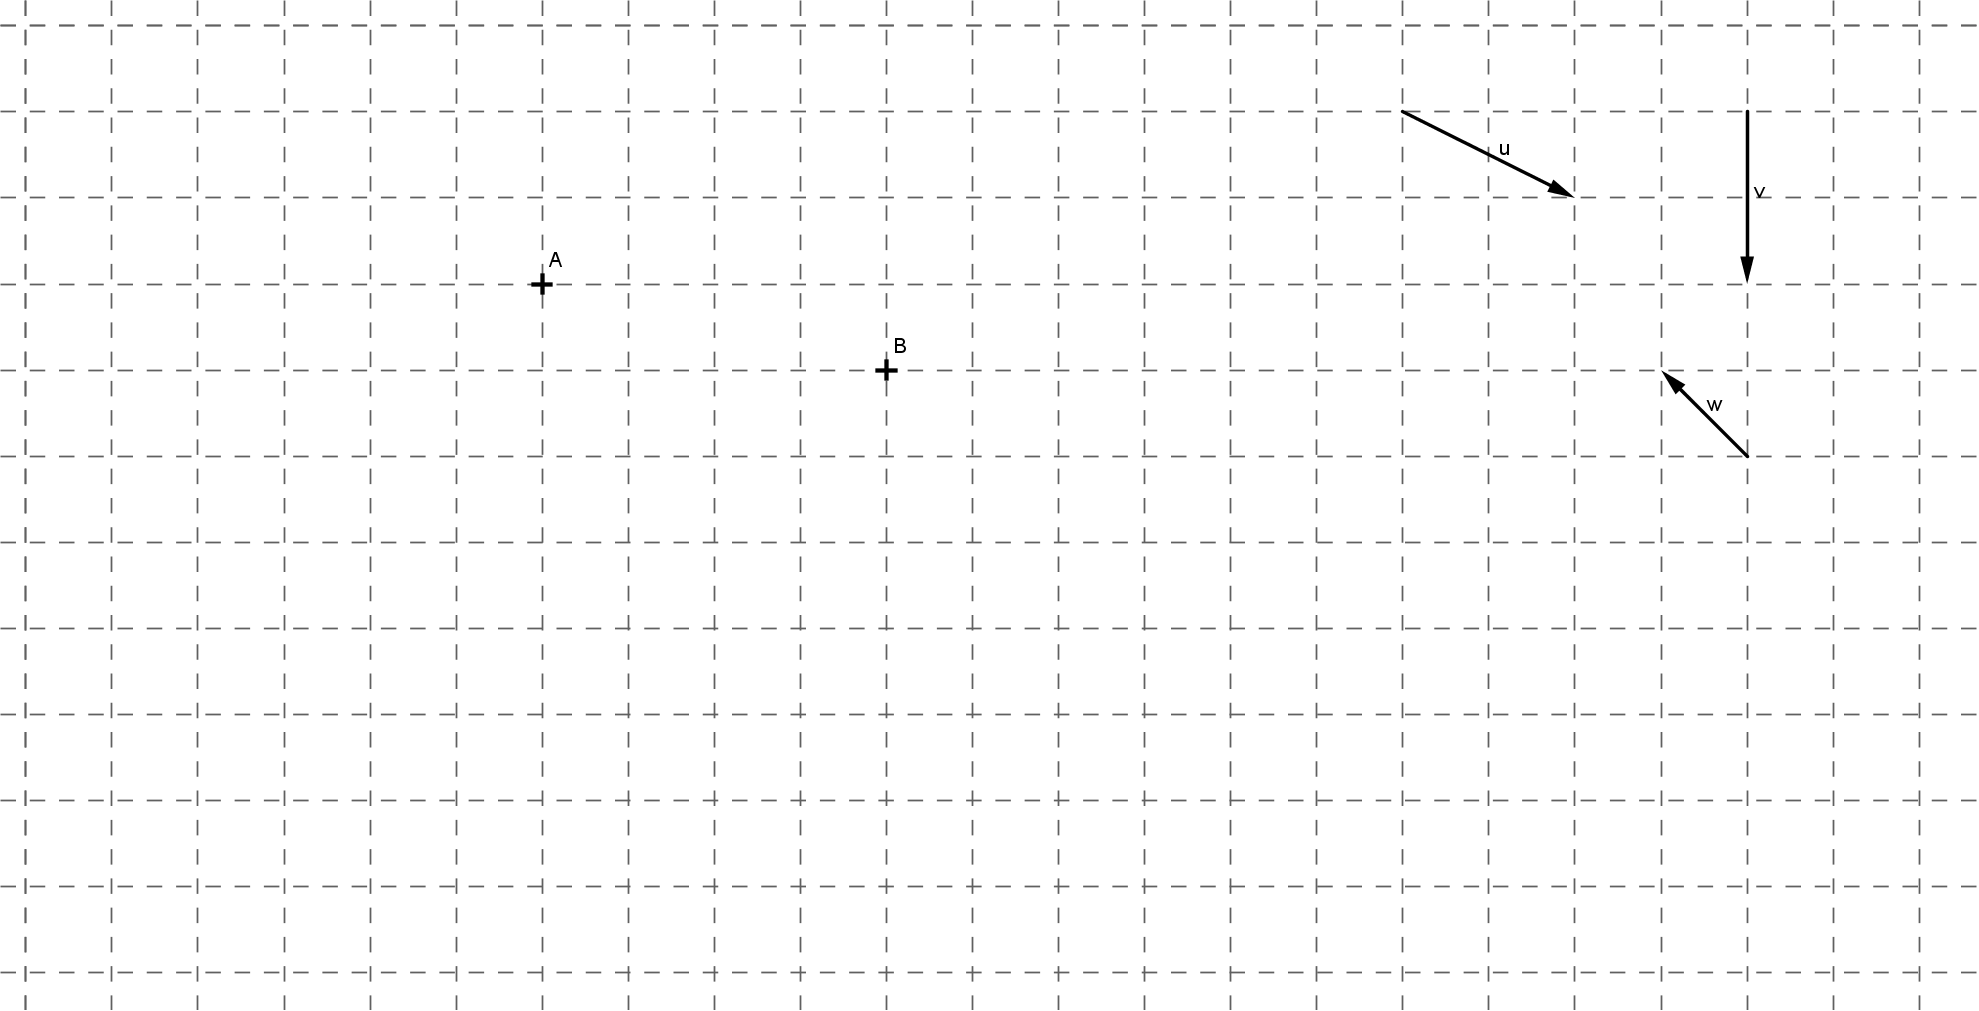
\includegraphics[width=17cm]{8bex1.png}
\end{center}
Placez les points C, D, E et F tels que :
$$\v{AC}=\v{u}+\v{v}+\v{w} \quad \quad \quad \quad \v{BD}=-\v{u}+\v{v}-\v{w} \quad \quad \quad \quad \v{AE}=3\v{u}+2\v{v} \quad \quad \quad \quad \v{EF}=\v{AB}-3\v{v}+4\v{w}$$
\end{EX}

\begin{EX}  En utilisant la relation de Chasles, simplifiez les écritures des $\v{u}$, $\v{v}$ et $\v{w}$ :
$$\v{u}=\v{AB}+\v{BC}+\v{CA} \quad \quad \quad \quad \v{v}=\v{AB}-\v{AC}+\v{BC}-\v{BA} \quad \quad \quad \quad \v{w}=\v{MA}-\v{MB}-\v{AB}$$
\end{EX}

\begin{EX} A et B sont deux points donnés. Soit C le point tel que : $3\v{AB}-2\v{AC}=\v{0}$
\begin{enumerate}
\item  Justifiez que $\v{AB}$ et $\v{AC}$ sont colinéaires.
\item Réalisez une figure avec les points A, B et C.
\end{enumerate}\end{EX}

\begin{EX} ABC est un triangle, tel que $AB=5$ , $AC=4$ et $BC=6$. \begin{enumerate}
\item Construire le point M tel que : $\v{AM}=\v{AB}+\v{AC}$.
\item Construire le point P tel que : $\v{MP}=\v{AB}+\v{CB}$.
\item \`A quel vecteur est égale la somme $\v{AM}+\v{MP}$ ?
\end{enumerate}
\end{EX}

\begin{EX} On considère un triangle ABC. \begin{enumerate}
\item Construire un représentant du vecteur $2\v{AB}$.
\item Construire un représentant du vecteur $-0,5\v{AC}$.
\item Construire le point D tel que $\v{AD}=2\v{BC}$.
\end{enumerate}
\end{EX}


\begin{EX} ABC est un triangle isocèle en A, tel que $AB=5$ , et $BC=4$. \begin{enumerate}
\item Construire le point M tel que : $\v{AM}=2\v{AB}+3\v{AC}$.
\item Construire le point P tel que : $\v{CP}=-\v{BC}+2\v{BA}$.
\end{enumerate}
\end{EX}


\newpage

\noindent\begin{minipage}{.20\linewidth}\begin{center}                  
\noindent \emph{Lycée Paul Lapie - Courbevoie}
\end{center}\end{minipage}
\begin{minipage}{1.5\linewidth}\begin{center}	
\noindent \cl\\ Chapitre 8
\end{center}\end{minipage}

\begin{center}\shadowbox{ \Large Planche n° 8 (ter) : Vecteurs et coordonnées } 	
\end{center}

\setcounter{EXO}{0} {\large{
\vfill
\begin{EX} 
Dans le repère $(O,\, I,\,J)$ ci contre, déterminer graphiquement les coordonnées des vecteurs $\v{OB}$, $\v{OC}$, $\v{DB}$, $\v{ED}$, $\v{DF}$, $\v{CE}$, $\v{DC}$, $\v{BA}$, $\v{AD}$, $\v{FB}$, $\v{EF}$.
\begin{center}
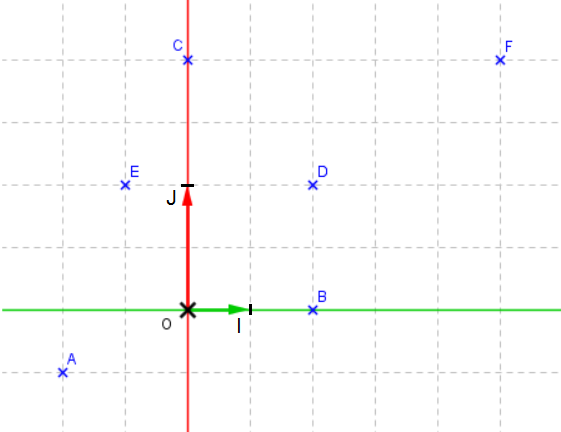
\includegraphics[width=10cm]{8tex1.PNG}
\end{center}
\end{EX}
\vfill
\begin{EX} 
Dans un repère, on donne les coordonnées des points :
$$A(3;\,2) \qquad B(2;\,1) \qquad C(4;\,-1) \qquad D(-2;\,-3)$$
Calculer les coordonnées des vecteurs suivants :
$$\v{AB} \qquad \qquad \qquad \v{CA} \qquad \qquad \qquad \v{DC} \qquad \qquad \qquad \v{BD} $$
\end{EX}
\vfill
\begin{EX} 
Soit un repère orthonormal $(O,\,I,\,J)$. On donne les coordonnées des quatres points :
$$E(-3;\,7) \qquad F(2;\,7) \qquad G(1;\,3) \qquad H(-4;\,3)$$
\begin{enumerate}
\item Calculez les coordonnées des vecteurs $\v{EF}$ puis $\v{HG}$.
\item Quelle est la nature du quadrilatère EFGH.
\end{enumerate}
\end{EX}
\vfill
\newpage
\begin{EX} Dans un repère, on donne les coordonnées des points :
$$A(1;\,4) \qquad \qquad B(4;\,6) \qquad \qquad D(4;\,3)$$
\begin{enumerate}
\item Calculer les coordonnées du vecteur $\v{AB}$.
\item  Calculer les coordonnées du point C tel que ABCD soit un parallélogramme.
\end{enumerate}
\end{EX}
\vfill
\begin{EX} Dans un repère, on donne les coordonnées des points :
$$B(7;\,1) \qquad \qquad C(3;\,0) \qquad \qquad D(1;\,3)$$
\begin{enumerate}
\item  Calculer les coordonnées du vecteur $\v{CB}$.
\item Calculer les coordonnées du point A tel que CBAD soit un parallélogramme.
\end{enumerate}

\end{EX}
\vfill
\begin{EX} A et B sont deux points donnés. Soit C le point tel que : $3\v{AB}-2\v{AC}=\v{0}$
\begin{enumerate}
\item  Justifiez que $\v{AB}$ et $\v{AC}$ sont colinéaires.
\item Réalisez une figure avec les points A, B et C.
\end{enumerate}
\end{EX}
\vfill
\begin{EX} Dans chacun des cas suivants, déterminez, si possible, le nombre $k$ tel que les vecteurs $\v{u}$ et $\v{v}$ soient colinéaires.
\begin{description}
\item [a.] $\v{u}=\left (\begin{array}{c}3 \\ -1 \\ \end{array} \right)$ et $\v{v}=\left (\begin{array}{c} k \\ 2 \\ \end{array} \right)$
\item [b.] $\v{u}=\left (\begin{array}{c}-2 \\ 5 \\ \end{array} \right)$ et $\v{v}=\left (\begin{array}{c} 1,5 \\ k \\ \end{array} \right)$
\item [c.] $\v{u}=\left (\begin{array}{c} -2 \\ 0 \\ \end{array} \right)$ et $\v{v}=\left (\begin{array}{c} k \\ 0 \\ \end{array} \right)$
\end{description}
\end{EX}
\vfill
\begin{EX} ABC est un triangle. I est le milieu de [AB], et J est le point tel que : $\v{AJ}=\v{AB}-2\v{AC}$.
\begin{enumerate}
\item Faites une figure.
\item  On choisit le repère (A ; $\v{AB}$ ; $\v{AC}$)
\begin{enumerate}
\item Quelles sont les coordonnées de I et J dans ce repère ?
\item Démontrez que (AJ) et (CI) sont parallèles.
\end{enumerate}
\end{enumerate}
\end{EX}
\vfill
}}



\newpage \setcounter{EXO}{0}

\noindent\begin{minipage}{.20\linewidth}\begin{center}                   % Lycée en haut à droite
\noindent \emph{Lycée Paul Lapie - Courbevoie}
\end{center}\end{minipage}
\begin{minipage}{1.5\linewidth}\begin{center}		% Classe  gauche
\noindent \cl\\ Chapitre 9
\end{center}\end{minipage}

\begin{center}\shadowbox{\large Planche n°9 : Statistiques } 		% Titre du chapître
\end{center}
\large
\begin{EX}
On a réalisé une enquête portant sur le nombre de livres lus pendant l'année par des élèves de seconde. Les résultats sont donnés ci-dessous :
~~\\
\begin{center}
\begin{tabular}{|p{5cm}| p{1cm}|p{1cm}|p{1cm}|p{1cm}|p{1cm}|p{1cm}|p{1cm}|p{1cm}|p{1cm}|}		% Taille des colonnes, nombre de colonnes
\hline							% Remplissage 1ère ligne
Nombre de livres lus & $1$&$2$&$3$&$4$&$5$&$6$ \\
\hline
Nombre d'élèves&$2$&$7$&$12$&$6$&$2$&$3$\\
\hline
\end{tabular}
\end{center}
~~\\
\begin{qu} Déterminez l'étendue de cette série.
\end{qu}

\begin{qu} Déterminez la médiane de cette série.
\end{qu}

\begin{qu} Déterminez le premier quartile et le troisième quartile de cette série.
\end{qu}

\begin{qu} Combien de livres un élève de cette classe lit-il en moyenne par an ?
\end{qu}

\begin{qu} Représentez cette série par un diagramme en bâtons.
\end{qu}

\end{EX}

\setcounter{ques}{0}
\begin{EX} Le graphique ci-dessous représente le polygone des fréquences cumulées croissantes des notes obtenues par les élèves d'une classe :
~~\\
\begin{center}
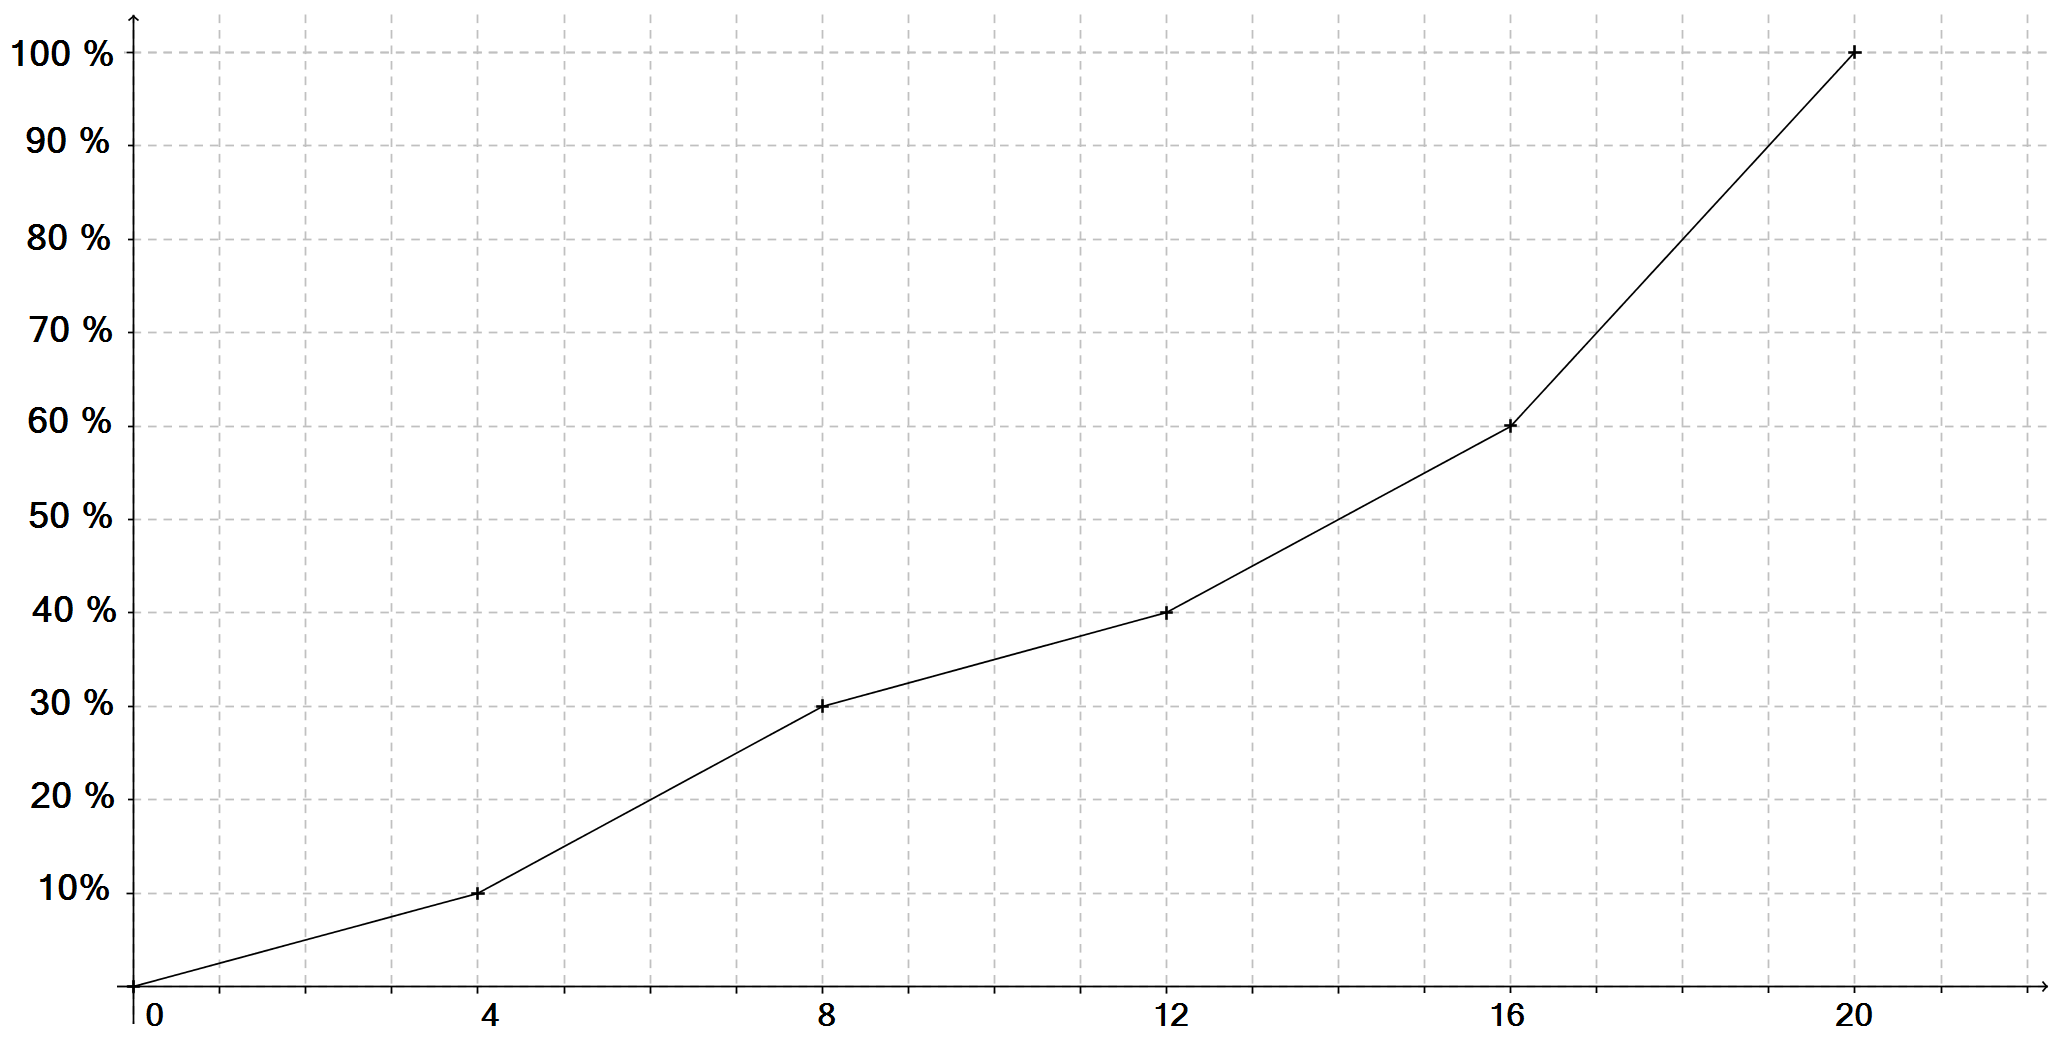
\includegraphics[width=15cm]{9ex2.png}
\end{center}
Complétez le tableau suivant :
\begin{center}
\begin{tabular}{|p{2cm}| p{2cm}|p{5.5cm}| p{6cm}|}		% Taille des colonnes, nombre de colonnes
\hline							% Remplissage 1ère ligne
Classe &Effectifs & Effectifs Cumulés Croissants & Fréquences Cumulées Croissantes \\
\hline
$[0;4[$&&&\\
\hline
$[4;8[$&&&\\
\hline
$[8;12[$&&&\\
\hline
$[12;16[$&&&\\
\hline
$[16;20[$&&&\\
\hline
Totaux&$30$&&\\
\hline
\end{tabular}
\end{center}
\end{EX}

\newpage
\setcounter{ques}{0}
\begin{EX}
Le tableau ci-dessous donne la répartition des notes obtenues à un contrôle de maths par 27 élèves d'une classe de seconde.
\begin{center}
\begin{tabular}{|p{2.1cm}|c|c|c|c|c|c|c|c|c|}		% Taille des colonnes, nombre de colonnes
\hline							% Remplissage 1ère ligne
Notes & $[1~;~3[$&$[3~;~5[$&$[5~;~7[$&$[7~;~9[$&$[9~;~11[$&$[11~;~13[$&$[13~;~15[$&$[15~;~17[$&$[17~;~19[$ \\
\hline
Effectifs&1&2&1&5&4&1&7&3&3\\
\hline
Effectifs Cumulés Croissants &&&&&&&&& \\
\hline
&&&&&&&&&\\
Fréquences&&&&&&&&&\\
&&&&&&&&&\\
\hline
 Fréquences Cumulées Croissantes&&&&&&&&&\\
\hline
\end{tabular}
\end{center}

\begin{qu} Calculez la note moyenne de cette classe.
\end{qu}

\begin{qu} Complétez le tableau.
\end{qu}

\begin{qu}
\begin{description}
\item [a.] Représentez graphiquement les fréquences cumulées croissantes.
\item [b.] Déterminez graphiquement la médiane, ainsi que les quartiles (Q1 et Q3).
\item [c.] Donnez l'intervalle inter-quartile.
\item [d.] Calculez l'écart inter-quartile et l'étendue.
\end{description}
\end{qu}
\end{EX}

\begin{EX}
Afin de renouveller le mobilier d'un lycée, le proviseur demande d'effectuer une enquête sur la taille de 100 élèves, voici le tableau obtenu, où les tailles sont exprimées en cm :\\
~~\\
\begin{center}
\begin{tabular}{|p{0.5cm}| p{0.5cm}|p{0.5cm}|p{0.5cm}|p{0.5cm}|p{0.5cm}|p{0.5cm}|p{0.5cm}|p{0.5cm}|p{0.5cm}|p{0.5cm}|p{0.5cm}|p{0.5cm}|p{0.5cm}|p{0.5cm}|p{0.5cm}|p{0.5cm}|p{0.5cm}|p{0.5cm}|p{0.5cm}|p{0.5cm}|}
\hline
$165$&$159$&$158$&$185$&$168$&$164$&$163$&$185$&$169$&$157$&$160$&$163$&$164$&$165$&$158$&$170$&$155$&$190$&$187$&$157$\\
\hline
$178$&$183$&$157$&$179$&$178$&$182$&$159$&$150$&$160$&$178$&$157$&$161$&$170$&$169$&$179$&$187$&$187$&$165$&$154$&$189$\\
\hline
$159$&$159$&$166$&$169$&$187$&$153$&$170$&$155$&$165$&$182$&$168$&$161$&$163$&$189$&$164$&$168$&$150$&$156$&$169$&$176$\\
\hline
$158$&$171$&$169$&$166$&$164$&$177$&$155$&$156$&$177$&$186$&$166$&$168$&$158$&$188$&$153$&$159$&$156$&$179$&$190$&$188$\\
\hline
$185$&$159$&$156$&$171$&$173$&$178$&$176$&$167$&$190$&$150$&$189$&$173$&$158$&$185$&$184$&$182$&$189$&$164$&$170$&$154$\\
\hline
\end{tabular}
\end{center}
~~\\
\begin{qu} Afin de faciliter le calcul de la moyenne, les données sont regroupées en classes. Complétez le tableau suivant puis calculez la moyenne de cette série.
\begin{center}
\begin{tabular}{|p{3cm}| p{2cm}|p{2cm}|p{2cm}|p{2cm}|p{2cm}|p{2cm}|}		
\hline							% Remplissage 1ère ligne
Classes & $[150~;~160[$&$[160~;~165[$&$[165~;~170[$&$[170~;~175[$&$[175~;~180[$&$[180~;~190[$ \\
\hline
Effectifs&&&&&&\\
\hline
\end{tabular}
\end{center}
\end{qu}

\begin{qu} Le calcul de la moyenne à l'aide des données a donné 169,3cm. Comparez cette valeur à celle obtenue à la question 1. Pouvez-vous expliquer cette différence ?
\end{qu}

\end{EX}
\newpage
\begin{EX} On a relevé les vitesses d'un certain nombre de voitures lors d'un contrôle routier. La série statistique obtenue est représentée par l'histogramme suivant :
\begin{center}
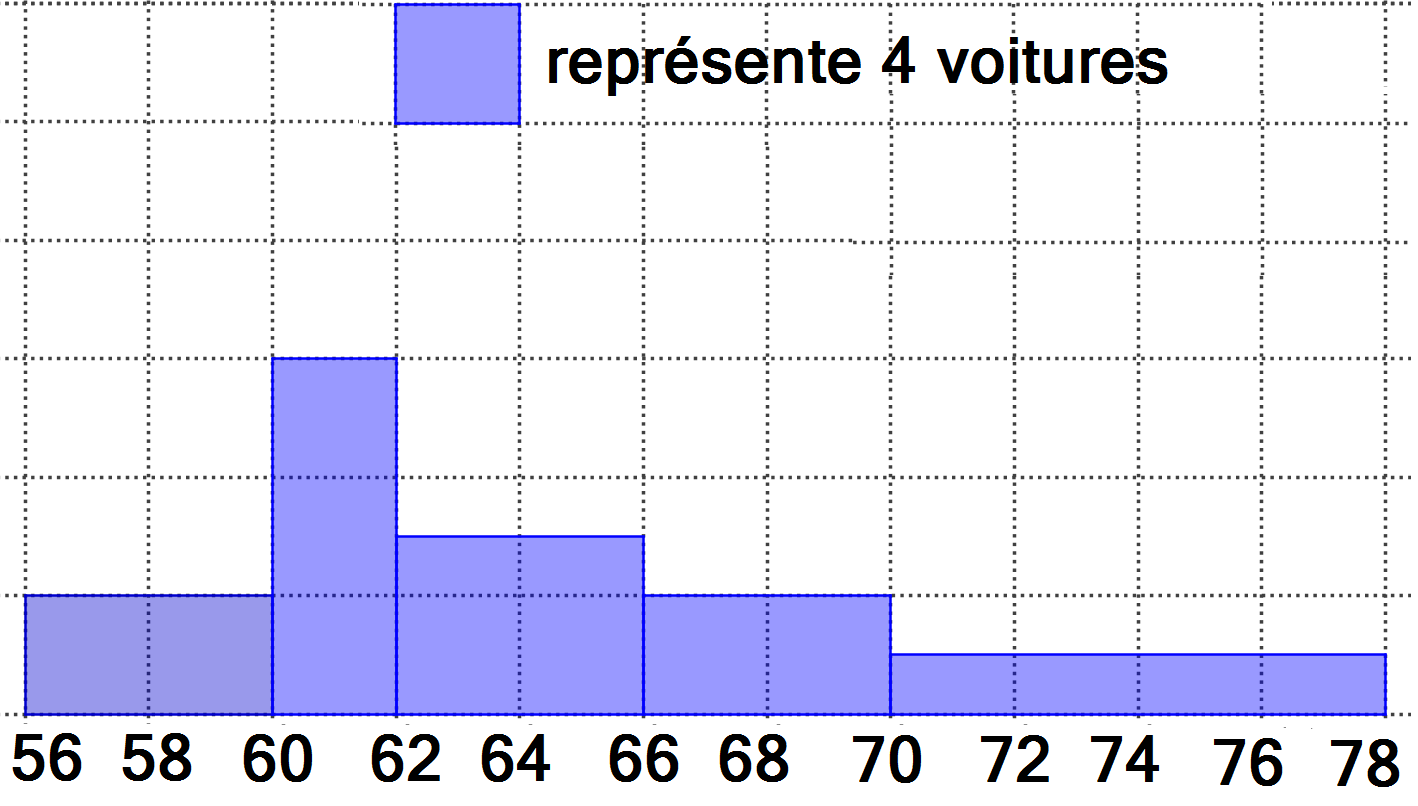
\includegraphics[width=10cm]{9ex5.png}
\end{center}
\begin{qu} Quel est le caractère étudié ?
\end{qu}

\begin{qu} Quelle est l'étendue de la série ?
\end{qu}

\begin{qu} Quel est l'effectif total de la série ?
\end{qu}

\begin{qu} Quelle est la classe médiane de la série ?
\end{qu}

\begin{qu} Complétez le tableau ci-dessous :
\begin{center}
\begin{tabular}{|p{3.5cm}| p{2cm}|p{2cm}|p{2cm}|p{2cm}|p{2cm}|p{2cm}|}		
\hline							% Remplissage 1ère ligne
Classes & $[56~;~60[$&$[60~;~64[$&&&$[72\,;\,78]$&Total \\
\hline
Effectifs&&&&$6$&&\\
\hline
Fréquences&&&&&&\\
\hline
FCC&&&&&&\\
\hline
Centres des classes&&&&&&\\
\hline
\end{tabular}
\end{center}
\end{qu}

\begin{qu} \`A quelle question répond-on quand on complète la case $(FCC ; [60~;~64[)$ ?
\end{qu}

\begin{qu} Calculez la vitesse moyenne des voitures lors de ce contrôle.
\end{qu}

\begin{qu} Tracez le polygone des fréquences cumulées croissantes et en déduire par lecture graphique une valeur approchée de la médiane, du premier et du troisième quartile.
\end{qu}

\end{EX}
\setcounter{ques}{0}
\begin{EX} Dans une même classe, les professeurs de Français et de Mathématiques comparent leurs notes :
\begin{center}
\begin{tabular}{|p{3cm}|p{0.5cm}| p{0.5cm}|p{0.5cm}|p{0.5cm}|p{0.5cm}|p{0.5cm}|p{0.5cm}|p{0.5cm}|p{0.5cm}|p{0.5cm}|p{0.5cm}|p{0.5cm}|p{0.5cm}|p{0.5cm}|p{0.5cm}|}		% Taille des colonnes, nombre de colonnes
\hline							% Remplissage 1ère ligne
Notes & $3$&$4$&$5$&$6$&$7$&$8$&$9$&$10$&$11$&$12$&$13$&$14$&$15$&$16$&$17$ \\
\hline
Effectifs Fr&0&0&0&0&3&5&3&7&6&3&2&1&0&0&0\\
\hline
Effectifs Maths&1&1&2&1&3&4&3&2&1&2&3&4&2&0&1\\
\hline
\end{tabular}
\end{center}
\begin{qu} Décrire la population et les caractères étudiés.
\end{qu}
\begin{qu} Représentez sur un même graphique les deux séries étudiées.
\end{qu}
\begin{qu} Quelle est l'étendue des deux séries étudiées ?
\end{qu}
\begin{qu} Calculez la moyenne en français et en maths.
\end{qu}
\begin{qu} Déterminez les médianes des deux séries.
\end{qu}
\begin{qu} Quelles conclusions peut-on donner à la comparaison ?
\end{qu}
\end{EX}

\begin{EX} Dans un lycée, le devoir commun de seconde en mathématiques a donné les résultats suivants :
\begin{center}
\begin{tabular}{|p{3.5cm}| p{2cm}|p{2cm}|p{2cm}|p{2cm}|p{2cm}|p{2cm}|}		
\hline							% Remplissage 1ère ligne
Classe & Seconde 1&Seconde 2&Seconde 3&Seconde 4&Seconde 5&Seconde 6 \\
\hline
Effectifs&35&31&34&32&35&16\\
\hline
Moyennes &$9,8$&$10,2$&$8,7$&$11,4$&$10,6$&$12,6$\\
\hline
\end{tabular}
\end{center}
Le professeur de mathématiques de la seconde 1 demande à ses élèves de calculer la moyenne de tous les élèves de seconde. Un élève donne très rapidement le résultat : $10,55$. \\

Que pensez-vous de ce résultat ?
\end{EX}

\begin{EX} Dans un groupe d'adolescents, la taille moyenne des garçons est de $1,74$m, et celle des filles $1,68$m.
\begin{qu} Peut-on calculer avec ces données seules la taille moyenne du groupe ?
\end{qu}
\begin{qu} Le groupe comporte 52 adolescents dont 31 filles. Calculer la taille moyenne du groupe arrondie au centième.
\end{qu}
\end{EX}

\begin{EX} Dans une entreprise A, le salaire moyen mensuel des hommes (qui représentent $50\%$ de l'effectif de l'entreprise) est de $1400$ euros, alors que celui des femmes est de $1000$ euros. 

Dans l'entreprise B,  le salaire moyen mensuel des hommes (qui représentent $20\%$ de l'effectif de l'entreprise) est de $1500$ euros, et celui des femmes est de $1110$ euros. 

Dans quelle entreprise le salaire moyen est-il le plus important ?

\end{EX}

\begin{EX} Une élève a eu $11,5$ de moyenne générale sur trois épreuves. Elle passe une quatrième épreuve. Chaque épreuve a pour coefficient 1. Sa moyenne générale sur ces quatre épreuves est égale à 11. 

Quelle note a-t-elle eu à la quatrième épreuve ? Justifiez votre réponse par un calcul.
\end{EX}
\newpage \normalfont
\begin{EX}
Dans un lycée on étudie les moyennes trimestrielles du premier trimestre de deux
classes de seconde, la seconde 1 et la seconde 2. 

\textbf{Partie A.} \\

Les 25 élèves de la seconde 1 ont obtenu les moyennes trimestrielles suivantes : \\
3 ; 4 ; 5 ; 7 ; 7 ; 10 ; 10 ; 10 ; 10 ; 10 ; 11 ; 11 ; 12 ; 12 ; 12 ; 12 ; 12 ; 13 ; 13 ; 13 ; 14 ; 15 ; 15 ; 16 ; 18.

\medskip

La moyenne trimestrielle de la classe s'obtient à partir des notes moyennes de
chaque élèves
\begin{enumerate}
\item Déterminer la médiane $M_e$, le premier quartile $Q_1$ et le troisième quartile $Q_3$ de cette série statistique de moyennes trimestrielles.
\item Représenter le diagramme en boîte correspondant en faisant apparaître les valeurs extrêmes.
\item Calculer la moyenne trimestrielle de la seconde 1.
\end{enumerate} 

\textbf{Partie B.} \\
 
Les indicateurs de la seconde 2 permettant de résumer la série statistique des
moyennes du premier trimestre sont les suivants : \\
Minimum = 3 ; $Q′_1 = 8$ ; $M′_e = 10$ ; $Q′_3 = 12$ ; maximum = 17 .
\begin{enumerate}
\item  Représenter, le diagramme en boîte correspondant en dessous de celui de la
classe jaune.
\item Parmi les affirmations suivantes, lesquelles sont vraies, fausses ou indécidables ?\\
\textit{(indécidable signifie que l’on ne peut pas conclure avec les éléments connus)} \\
Justifier votre réponse dans chacun des cas. \begin{enumerate}
\item $50 \%$ des élèves de la seconde 2 ont une note comprise entre 10 et 12.
\item $75 \%$ des élèves de la seconde 2 ont une note inférieure ou égale à 12.
\item Au moins $50 \%$ des élèves de la seconde ont une note inférieure ou
égale à la note médiane de la série de la seconde 1.
\end{enumerate}\end{enumerate}
\end{EX}

\begin{EX}
\textit{Dans tout l'exercice les poids sont exprimés en grammes.}

On effectue un prélèvement de 57 paquets de farine sur une chaîne
de production. Les 57 poids relevés sont donnés dans le tableau ci-dessous: 

\begin{center}
\begin{tabular}{|p{2.5cm}| p{0.7cm}| p{0.7cm}|p{0.7cm}| p{0.7cm}|p{0.7cm}| p{0.7cm}|p{0.7cm}| p{0.7cm}|p{0.7cm}| p{0.7cm}|p{0.7cm}| p{0.7cm}|p{0.7cm}|}		
\hline	
  \cline{1-14}
   Poids en g. &495 &497 &499 &500 &501 &502 &503 &505 &506 &507 &508 &509 &512\\
   \cline{1-14}
   Effectif & 1&2&3&5&5&7&9&8&7&5&2&2&1\\
   \cline{1-14}
   ECC & & & & & & & & & & & & & \\
    \cline{1-14}
\end{tabular}\end{center}

\begin{enumerate}
\item Calculer la moyenne des poids de ces 57 paquets de farine. On arrondira
cette valeur au dixième. 
\item Compléter la ligne des effectifs cumulés croissants dans le tableau
précédent. 
\item Déterminer la médiane des poids de ces 57 paquets de farine. 
\item Parmi tous ces poids, déterminer le plus petit poids $P$ pour lequel
au moins trois quarts des paquets ont un poids inférieur ou égal à 
$P$ (en grammes). Quel paramètre de la série a-t-on ainsi trouvé ? 
\item Calculer le pourcentage, à 0,1 \% près, des paquets ayant un poids inférieur ou égal
à  $499$ grammes.
\item Calculer la fréquence des paquets dont le poids est égal à  505 grammes. 
\item On suppose maintenant que le dernier poids est 612 grammes au lieu
de 512 grammes. Donner alors la valeur de la médiane et de $Q_{3}$. 
\item On suppose maintenant que tous les poids sont augmentés de 100 grammes
par rapport au tableau (les poids sont donc 595, 597, ... , 609, 612).
Que devient alors la valeur de la médiane? Et de la moyenne ?
\end{enumerate}
\end{EX}





\newpage \setcounter{EXO}{0}


\noindent\begin{minipage}{.20\linewidth}\begin{center}                  
\noindent \emph{Lycée Paul Lapie - Courbevoie}
\end{center}\end{minipage}
\begin{minipage}{1.5\linewidth}\begin{center}	
\noindent \cl\\ Chapitre 10
\end{center}\end{minipage}

\begin{center}\shadowbox{ \Large Planche n° 10 : \'Equations de droites } 	
\end{center}
{\small{
\begin{EX}
Lire graphiquement les équations des droites ci-dessous :
\begin{center}
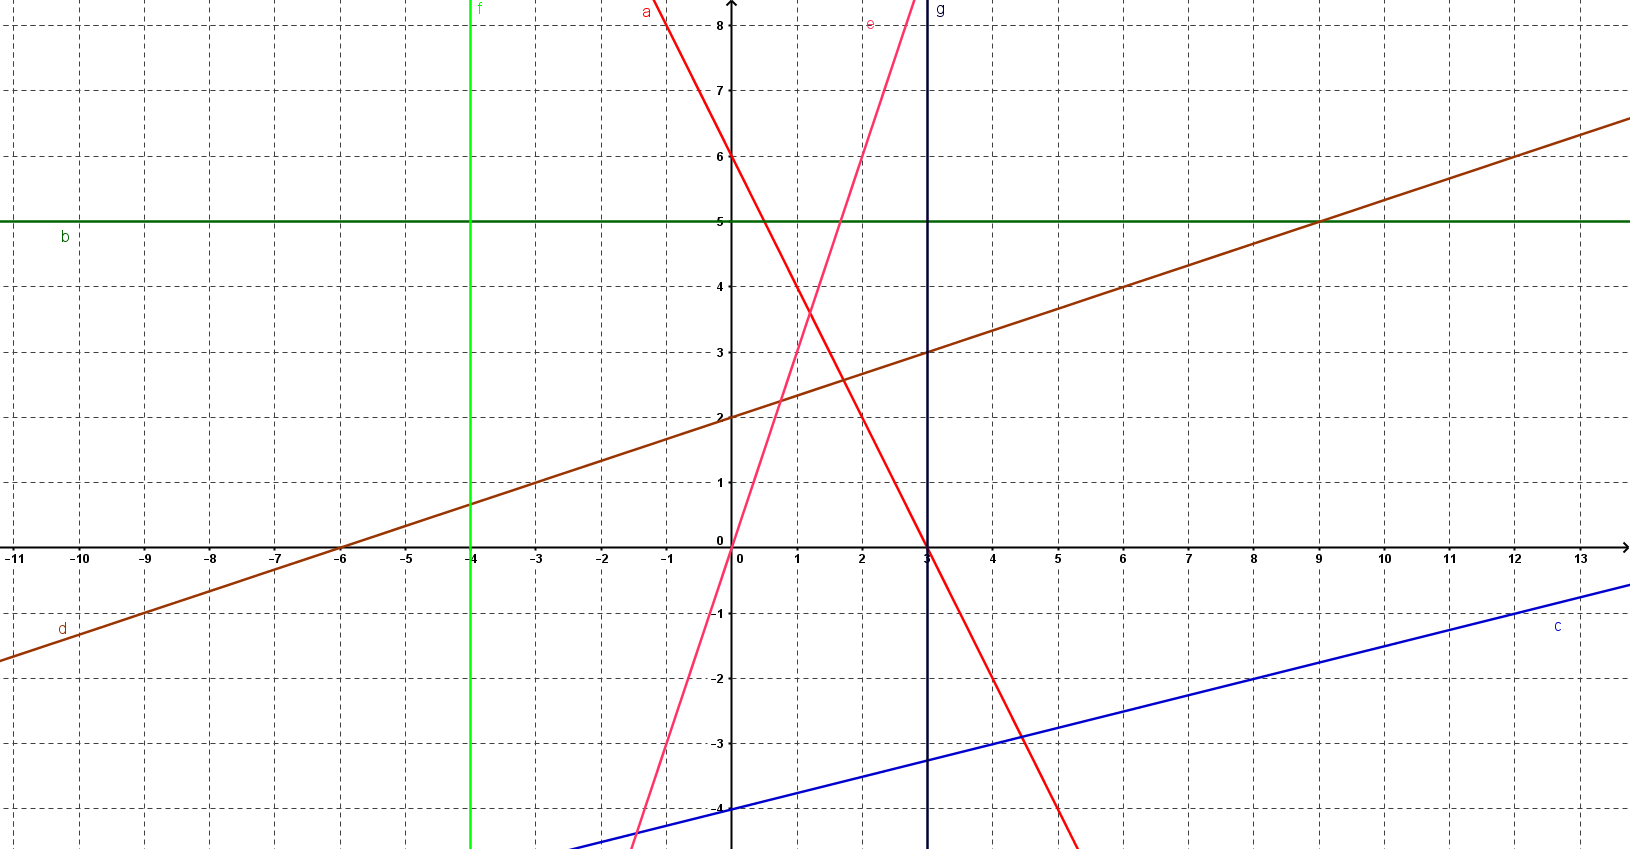
\includegraphics[width=12cm]{10ex3.png}
\end{center}
\end{EX}

\begin{EX}
Dans chacun des cas suivant, déterminer les coordonnées du point d'intersection de la droite $(d)$ avec l'axe des abscisses. 
$$d:y=\f{2}{3}x-6 \qquad d:y=4x+7 \qquad d: 3x-5y=8 \qquad d:x=-3$$
\end{EX}

\begin{EX}
Dans chacun des cas suivant, le point $A$ appartient à la droite $(d)$. Déterminer alors la valeur du réel $t$:
\begin{center} $A(t,1)$ et $d:x=7$
\qquad \qquad$A(-3,4)$ et $d:x=t$
\qquad \qquad $A(4,3)$ et $d:y=3x-t$ \\ $A(-7,11)$ et $d:y=tx+8$
\qquad \qquad$A(t,-6)$ et $d:y=3x+t$
\end{center}
\end{EX}
\begin{EX}
\renewcommand{\tabularxcolumn}[1]{b{#1}}
\begin{tabularx}{\linewidth}{Xc}	
On considère la figure ci-dessous. Les deux rectangles ABCD et EFGH ont le même centre (intersection des diagonales).

~~

~~ \vspace{1cm}

~~

Les droites $(AE)$ et $~(CG)$ sont-elles confondues ?

~~

~~ \vspace{1cm}


&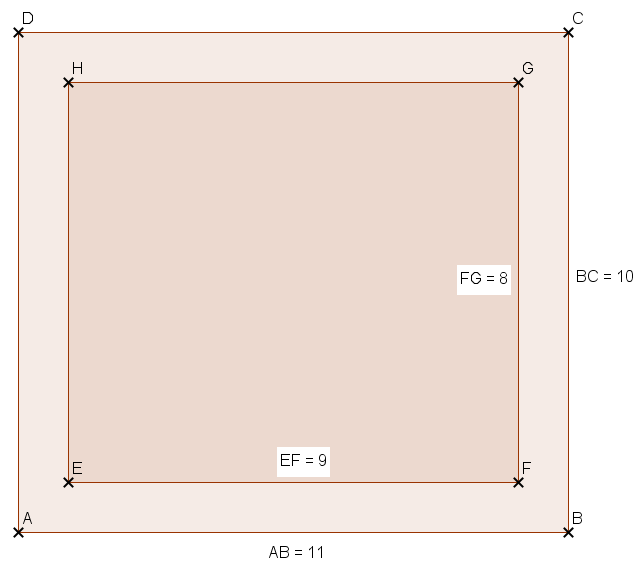
\includegraphics[width=5cm]{10ex1.png}
\end{tabularx}

\end{EX}

\begin{EX}\renewcommand{\tabularxcolumn}[1]{b{#1}}
\begin{tabularx}{\linewidth}{Xc}	
Dans le repère orthonormé $(O\,;\,I\,;\,J)$ suivant, déterminer les coordonnées des points B, C et D.

~~

~~ \vspace{2cm}

~~



&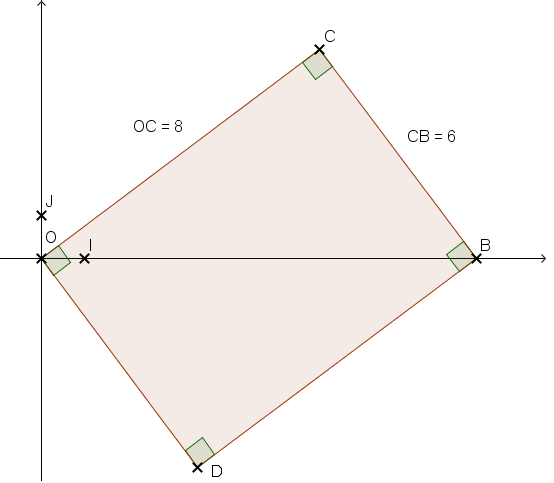
\includegraphics[width=6cm]{10ex2.png}
\end{tabularx}

\end{EX}
}}
\newpage \setcounter{EXO}{0}
\noindent\begin{minipage}{.20\linewidth}\begin{center}                  
\noindent \emph{Lycée Paul Lapie - Courbevoie}
\end{center}\end{minipage}
\begin{minipage}{1.5\linewidth}\begin{center}	
\noindent \cl\\ Chapitre 10
\end{center}\end{minipage}

\begin{center}\shadowbox{ \Large Planche n° 10 (bis) : \'Equations de droites} 	
\end{center}

\begin{EX}
Soit $d$ la droite d'équation cartésienne : $2x-3y+1=0$. 
\begin{enumerate}
\item Déterminer un point et un vecteur directeur de $d$. 
\item Le point $B(7\,;\,5)$ appartient-il à la droite $d$ ? Justifier ?
\end{enumerate}

\end{EX}

\begin{EX} Soient deux points $A(4\,;\,-1)$ et $B(-3\,;\,5)$.
\begin{enumerate}
\item Déterminer les coordonnées d'un vecteur directeur de la droite $(AB)$.
\item En utilisant l'équivalence : $M \in (AB) \ssi \v{AM} \text{ et } \v{AB} \text{ sont colinéaires}$, déterminer une équation cartésienne de la droite $(AB)$.
\item Déterminer une équation cartésienne de la droite parallèle à $(AB)$ et passant par $C(1\,;\,-2)$.
\end{enumerate}

\end{EX}

\begin{EX}
Déterminer une équation cartésienne des droites suivantes :
\begin{enumerate}
\item passant par $A(2\,;\,4)$ et $B(5 \,;\,-1)$
\item passant par $C(3\,;\,4)$ et de vecteur directeur $\v{u}\left (\begin{array}{c}
2	 \\
	1 \\
\end{array} \right)$.
\item passant par $D(7\,;\,2)$ et parallèle à la droite $(EF)$ avec $E(1\,;\,1)$ et $F(4\,;\, 0)$.
\end{enumerate}

\end{EX}

\begin{EX} Déterminer le ou les points d'intersection des droites suivantes : 
$$(d):\quad 2x-3y+4=0 \hspace{2cm} (d'):\quad x+2y-1=0$$

\end{EX}
\begin{EX} Déterminer le ou les points d'intersection des droites suivantes : 
$$(d):\quad -x+10y+1=0 \hspace{2cm} (d'):\quad 2x+5y-8=0$$

\end{EX}
\begin{EX} Déterminer le ou les points d'intersection des droites suivantes : 
$$(d):\quad 4x-5y+3=0 \hspace{2cm} (d'):\quad 2x+y-1=0$$

\end{EX}
\begin{EX} On considère la droite $(d)$ d'équation réduite : 
$$y=2x-4$$
\begin{enumerate}
\item Déterminer une équation cartésienne de $(d)$.
\item Donner un point de $(d)$ et un vecteur directeur de $(d)$.
\end{enumerate}
\end{EX}






\newpage \setcounter{EXO}{0}
\noindent\begin{minipage}{.20\linewidth}\begin{center}                  
\noindent \emph{Lycée Paul Lapie - Courbevoie}
\end{center}\end{minipage}
\begin{minipage}{1.5\linewidth}\begin{center}	
\noindent \cl\\ Chapitre 10
\end{center}\end{minipage}

\begin{center}\shadowbox{ \Large Planche n°10 : \'Equations de droites } 	
\end{center}

\begin{EX}
Soit $d$ la droite d'équation cartésienne : $3x+5y-2=0$. 
\begin{enumerate}
\item Déterminer un point et un vecteur directeur de $d$. 
\item Le point $B(9\,;\,-5)$ appartient-il à la droite $d$ ? Justifier ?
\end{enumerate}

\end{EX}

\begin{EX} Soient deux points $A(7\,;\,-3)$ et $B(4\,;\,1)$.
\begin{enumerate}
\item Déterminer les coordonnées d'un vecteur directeur de la droite $(AB)$.
\item En utilisant l'équivalence : $M \in (AB) \ssi \v{AM} \text{ et } \v{AB} \text{ sont colinéaires}$, déterminer une équation cartésienne de la droite $(AB)$.
\item Déterminer une équation cartésienne de la droite parallèle à $(AB)$ et passant par $C(2\,;\,-2)$.
\end{enumerate}

\end{EX}

\begin{EX}
Déterminer une équation cartésienne des droites suivantes :
\begin{enumerate}
\item passant par $A(3\,;\,5)$ et $B(2 \,;\,1)$
\item passant par $C(2\,;\,-4)$ et de vecteur directeur $\v{u}\left (\begin{array}{c}
-3 \\
	4 \\
\end{array} \right)$.
\item passant par $D(2\,;\,-3)$ et parallèle à la droite $(EF)$ avec $E(1\,;\,-1)$ et $F(4\,;\, 2)$.
\end{enumerate}

\end{EX}




\newpage \setcounter{EXO}{0}


\noindent\begin{minipage}{.20\linewidth}\begin{center}                  
\noindent \emph{Lycée Paul Lapie - Courbevoie}
\end{center}\end{minipage}
\begin{minipage}{1.5\linewidth}\begin{center}	
\noindent \cl\\ Chapitre 11
\end{center}\end{minipage}

\begin{center}\shadowbox{ \Large Planche n° 11 : Probabilités } 	
\end{center}
\begin{EX}
Un club de vacances comprend cent touristes. Un sondage donne les résultats suivants :
\begin{center}
\begin{tabular}{|p{4cm}| p{4cm}| p{4cm}|}		
\hline							
 & Homme & Femme \\
\hline
Pratique un sport & 48 & 12\\
\hline
Ne pratique pas de sport & 16 & 24\\
\hline
\end{tabular}
\end{center}
On choisit un touriste au hasard.
\begin{qu} Quelle est la probabilité ... \begin{itemize} \item que ce soit un homme ? \item que ce soit une femme ? \item qu'il pratique du sport ? \item que ce soit une femme qui ne pratique pas de sport ? \end{itemize}
\end{qu}
\begin{qu} On choisit un touriste parmi les femmes. Quelle est la probabilité qu'elle ne pratique pas de sport ?
\end{qu}
\end{EX}
\begin{EX}
Dans un magasin, les modes de paiement et les montants des achats sont répartis de la façon suivante :
\begin{itemize}
\item 50 \% des achats ont été payés par chèque;
\item 70 \% des achats sont d'un montant inférieur ou égal à 200 euros, dont 20 \% sont réglés en espèces;
\item 15 \% des achats sont réglés par carte banquaires et sont d'un montant inférieur ou égal à 200euros;
\item 2 \% des achats sont d'un montant supérieur à 200 euros et sont réglés en espèces.
\end{itemize}

\begin{qu}
Recopiez et complétez le tableau ci-dessous : ( on note M le montant des achats)
\begin{center}
\begin{tabular}{|p{4cm}| p{3cm}|p{3cm}|p{3cm}|}		% Taille des colonnes, nombre de colonnes
\hline							% Remplissage 1ère ligne
Mode de paiement & $M \ie 200$ & $ M>200$ & Total \\
\hline
Espèces & & &  \\
\hline
Chèque & & & \\
\hline
Carte & & & \\
\hline
Total & & & \\
\hline
\end{tabular}
\end{center}

\end{qu}

\begin{qu}
On prend au hasard un bordereau d'achat. Calculez les probabilités des événements : 
\begin{itemize}
\item A: \og L'achat dépasse 200 euros \fg
\item B: \og L'achat est réglé par carte banquaire ou par chèque \fg
\item C: \og L'achat est réglé par carte \fg 
\end{itemize}
\end{qu}

\end{EX}
\begin{EX}
Stéphane a deux pantalons : un noir et un bleu; trois chemises : une bleue, une jaune et une noire; et deux vestes : une bleue et une marron.

On suppose que Stéphane choisit au hasard un pantalon, puis une chemise, puis une veste. On notera $P_N$ et $P_B$ les pantalons respectivement noir et bleu, $C_B$, $C_J$ et $C_N$ les chemises, puis $V_B$ et $V_M$ les vestes. 
\begin{qu} Dressez un arbre de probabilité représentant toutes les tenues qu'il pourrait porter. Combien y a-t-il d'issues ?
\end{qu}

\begin{qu} On considère l'événement A:\og Il porte une chemise et une veste bleues \fg. Quelle est la probabilité de l'événement A, p(A) ?
\end{qu}

\begin{qu} On considère l'événement B :\og Il porte du noir \fg. Quelle est la probabilité de l'événement B, p(B) ?
\end{qu}

\begin{qu} \'Enoncez l'événement contraire $\bar B$ puis calculez sa probabilité, p($\bar B$).
\end{qu}

\begin{qu} \'Enoncez un événement C dont la probabilité est $p(C)=\displaystyle{ \frac{6}{18}=\frac{1}{3}}$. Quelles sont les issues réalisant cet événement ?
\end{qu}

\end{EX}
\begin{EX}
Dans un groupe de $60$ personnes, $34$ aiment le rap, $36$ ont moins de $20$ ans, et parmi ces $36$ jeunes personnes, $26$ aiment le rap. On rencontre au hasard une personne de ce groupe.
\begin{qu} Soit l'événement J: \og la personne a moins de $20$ ans\fg. Calculer $p(J)$. En déduire la probabilité de l'événement contraire à J.
\end{qu}
\begin{qu} Reproduire et compléter le tableau croisé suivant :
\begin{center}
\begin{tabular}{|p{4cm}| p{4cm}| p{4cm}| p{4cm}|}		
\hline							
 & Moins de $20$ ans & $20$ ans ou plus & Total \\
\hline
Aime le rap & & &\\
\hline
N'aime pas le rap & & &\\
\hline
Total & & &\\
\hline
\end{tabular}
\end{center}
\end{qu}
\begin{qu} Soit l’événement R : « La personne n’aime pas le rap et a moins de 20 ans» . Déterminer la
probabilité de l’événement R.
\end{qu}
\begin{qu}
On notera C « La personne n’aime pas le rap sachant qu’elle est jeune» .
La personne rencontrée est un jeune de moins de 20 ans, quelle est la probabilité que cette
personne n’aime pas le rap ?
\end{qu}

\end{EX}
\begin{EX}
Une entreprise fabrique des outils. On analyse 500 outils à la sortie de la chaîne de fabrication et on décèle deux types de défauts, un défaut de calibrage noté Défaut C et un défaut de résistance noté Défaut R. On a observé que 21 outils présentaient le défaut de calibrage, dont 9 présentaient aussi le défaut de résistance. De plus, 75 outils avaient le défaut de résistance sans avoir celui de calibrage.

\begin{qu}
Reproduire et compléter le tableau croisé ci-dessous :
\begin{center}
\begin{tabular}{|p{4cm}| p{4cm}| p{4cm}| p{4cm}|}		
\hline							
 & Défaut C & Pas de défaut C & Total \\
\hline
Défaut R & & &\\
\hline
Pas de défaut R & & &\\
\hline
Total & & &\\
\hline
\end{tabular}
\end{center}
\end{qu}
\begin{qu} On prélève au hasard un outil dans le lot des 500 outils étudiés. Quelle est la probabilité des évènements suivants : \\
- A = « L'outil ne présente pas le défaut de calibrage » ,\\
- B = « L'outil ne présente aucun des deux défauts » ,\\
- D = « L'outil présente au moins un des deux défauts » .
\end{qu}
\begin{qu} On prélève au hasard un outil parmi ceux qui présentent un défaut de résistance. Quelle est la probabilité qu'il ne présente pas le défaut de calibrage ?
\end{qu}

\end{EX}
\begin{EX}

Une urne contient 70 boules blanches et 30 boules noires. Toutes les boules étant
indiscernables au toucher, on tire au hasard une première boule qu’on remet ensuite dans
l’urne avant de tirer une seconde boule. On s’intéresse aux deux couleurs obtenues.
\begin{qu}  Réaliser un arbre pour modéliser cette expérience aléatoire.
\end{qu}
\begin{qu}Calculer les probabilités des événements suivants : \\
$A$ : « les deux boules sont blanches ». \\
$B$ : « les deux boules sont de la même couleur ».
\end{qu}

\end{EX}
\begin{EX}		

On tire au hasard dans un jeu de 32 cartes. On considère les événements suivants : \\
$A$ : « La carte obtenue est un carreau » ;\\
$B$ : « La carte obtenue est un as »
\begin{qu} Calculer $p(A)$ et $p(B)$.
\end{qu}
\begin{qu} Définir, à l’aide d’une phrase en français, l’événement $A\cap B$. Calculer $p(A\cap B)$.
\end{qu}
\begin{qu} Soit $C$ défini par : « La carte obtenue est un carreau ou un as». Calculer $p(C)$.
\end{qu}


\end{EX}
\begin{EX}

On lance deux fois de suite un dé équilibré dont les six faces sont numérotées de 1 à 6 et on s’intéresse à la somme des points obtenus. \\

On considère l’événement S : « La somme des deux nombres obtenus est supérieure à 9 ».
Calculer la probabilité p(S).


\end{EX}
\begin{EX}

On joue avec un dé truqué à 6 faces, numérotées de 1 à 6.
On lance une fois le dé et on s’intéresse au numéro de la face du dessus.
Le tableau suivant indiquent les probabilités des événements élémentaires :

\begin{center}
\begin{tabular}{|p{1.8cm}| p{0.7cm}| p{0.7cm}| p{0.7cm}| p{0.7cm}| p{0.7cm}| p{0.7cm}|}		
\hline							
Issues & 1&2&3&4&5&6\\
\hline
Probabilités & 0,2& 0,1 &0,1 &0,1& 0,2& 0,3\\
\hline
\end{tabular}
\end{center}

\begin{qu}Soit A l’événement : «obtenir un nombre supérieur à 3».
Donner A sous forme d’ensemble d’issues puis calculer $p(A)$.
\end{qu}
\begin{qu} Soit l’événement B : «obtenir un nombre pair».
Donner B sous forme d’ensemble d’issues puis calculer $p(B)$.
\end{qu}
\begin{qu} \begin{description}
\item [a.] Décrire l'événement $A \cap B$, le donner sous forme d’ensemble d’issues puis calculer $p(A\cap B)$.
\item [b.] Déduire de ce qui précède la probabilité $p(A\cup B)$.
\end{description}
\end{qu}

\end{EX}
\begin{EX}
Le jeu du loto est constitué d'une grille contenant 49 numéros, de 1 à 49 ; et une grille de $10$ chiffres, de $1$ à $10$. Lors du tirage du loto, $5$ numéros parmi la grille de $49$ sont tirés, et $1$ numéro parmi la grille de $10$, appelé le \og numéro chance\fg.

Quelle est la probabilité d'obtenir le bon tirage ? On donnera le résultat sous forme de pourcentage.
\end{EX}

\begin{EX}
Une production en très grande série contient $90$\% de pièces conformes, les autres étant des pièces déféctueuses. Un contrôle de qualité accepte les pièces conformes dans $92$\% des cas, et rejette les pièces déféctueuses dans $94$\% des cas.\\

Après le contrôle de qualité, on tire une pièce au hasard dans la production. On note C l'événement \og La pièce est conforme\fg \, et A l'événement \og La pièce est acceptée par le contrôle de qualité\fg.
\begin{qu} Contruire un arbre de probabilité complet.
\end{qu}
\begin{qu} Donner la probabilité que la pièce tirée soit ... \begin{description}
\item [a.] conforme et acceptée par le contrôle;
\item [b.] conforme et rejetée par le contrôle;
\item [c.] défectueuse  et acceptée par le contrôle;
\item [d.] défectueuse  et rejetée par le contrôle; \end{description}
\end{qu}
\begin{qu} En déduire la probabilité que la pièce prelevée ait subi une erreur de contrôle.
\end{qu}
\end{EX}

\begin{EX}

Voici les noms de footballeurs qui ont obtenu le ballon d'or. 
\begin{center} {\emph{Cruyff \quad Beckenbauer \quad Platini \quad Weah \quad Zidane \quad Figo \quad Ronaldinho \quad Cannavaro \quad Messi \quad Ronaldo}} \end{center}

On prélève au hasard un nom de cette liste.
\begin{qu} Quelle est la probabilité que le nom comporte strictement moins de 6 lettres ?
\end{qu}
\begin{qu} Quelle est la probabilité que le nom ne comporte pas la lettre A ?
\end{qu}
\end{EX}


\newpage \setcounter{EXO}{0}

\noindent\begin{minipage}{.20\linewidth}\begin{center}                  
\noindent \emph{Lycée Paul Lapie - Courbevoie}
\end{center}\end{minipage}
\begin{minipage}{1.5\linewidth}\begin{center}	
\noindent \cl\\ Chapitre 13
\end{center}\end{minipage}

\begin{center}\shadowbox{ \Large Planche n° 13 : \'Echantillonnage et estimation } 	
\end{center}

\begin{EX}
Léa et Léo ont chacun une pièce de 1 euro. Léa lance 50 fois sa pièce et obtient 19 fois pile. Léo lance 100 fois sa pièce et obtient 38 fois pile. 
\begin{qu} Montrez que la fréquence d'apparition de pile est égale pour chacun d'entre eux. 
\end{qu}
Léa et Léo en déduisent que leurs deux pièces sont très probablement déséquilibrées. 
\begin{qu} En utilisant les intervalles de confiance, expliquez que leur conclusion est discutable.
\end{qu}
\end{EX}

\begin{EX}
Après avoir pêché 100 poissons dans un lac, je constate que j'ai obtenu 37 brochets.
\begin{qu} Je fais l'hypothèse qu'il y a une proportion p de brochets dans le lac. Dans chacun des cas suivants, indiquez si mon hypothèse peut être acceptée à l'aide de l'intervalle de fluctuation au seuil $95\%$. 
\begin{center}
a) p=0,4 \hspace{3cm} b) p=0,28 \hspace{3cm} c) p=0,48
\end{center}
\end{qu}
\begin{qu} Indiquer l'ensemble des valeurs de $p$ qui pourraient être acceptées suite à cet échantillonnage.
\end{qu}
\end{EX}

\begin{EX}Une entreprise annonce que le pourcentage de moteurs défectueux dans la production est égal à $1\%$. Afin de vérifier cette affirmation, $800$ moteurs sont prélevés au hasard. On constate que 15 moteurs sont détectées défectueux.\\

Le résultat de ce test remet-il en question l'annonce de l'entreprise ? Justifier.\\
\textit{Vous déterminerez l'intervalle de confiance obtenu à partir de la fréquence observée, puis vous argumenterez pour répondre à la question.}
\end{EX}

\begin{EX}
Une association de consommateurs décide d’estimer la proportion de personnes satisfaites par l’utilisation d’une crème. Elle réalise un sondage parmi les personnes utilisant ce produit. Sur 140 personnes interrogées, 99 se déclarent satisfaites.

Estimer, par intervalle de confiance, la proportion de personnes satisfaites parmi les utilisateurs de la crème.
\end{EX}

\begin{EX}
Voici les résultats d’un sondage IPSOS réalisé avant l’élection présidentielle de
2002 pour Le Figaro et Europe 1, les 17 et 18 avril 2002 auprès de 989 personnes,
constituant un échantillon national représentatif de la population française âgée
de 18 ans et plus et inscrite sur les listes électorales. \\
On suppose cet échantillon constitué de manière aléatoire (même si en pratique
cela n’est pas le cas). Les intentions de vote au premier tour pour les principaux
candidats sont les suivantes : 
\begin{center}
Jacques Chirac : $20 \%$ \hspace{2cm} Lionel Jospin : $18 \%$  \hspace{2cm}  Jean-Marie Le Pen : $14 \%$.
\end{center}
Les médias se préparent pour un second tour entre Jacques Chirac et Lionel Jospin.
\begin{qu} Déterminer, pour chaque candidat, l'intervalle de confiance de la proportion inconnue d'électeurs ayant l'intention de voter pour lui.
\end{qu}
\begin{qu} Le 21 avril, les résultats du premier tout des élections sont les suivants :
\begin{center}
J. Chirac : $19,88 \%$ \hspace{2cm} L. Jospin : $16,18 \%$  \hspace{2cm}  J-M. Le Pen : $16,86 \%$.
\end{center}
Les pourcentages de voix recueillies par chaque candidat sont-ils bien dans les intervalles de confiance précédents ?
\end{qu}
\begin{qu} Pouvait-on, au vu de ce sondage, écarter l'un des trois candidats au second tour ?
\end{qu}
\end{EX}



\end{document}		% Le document se termine ici.
